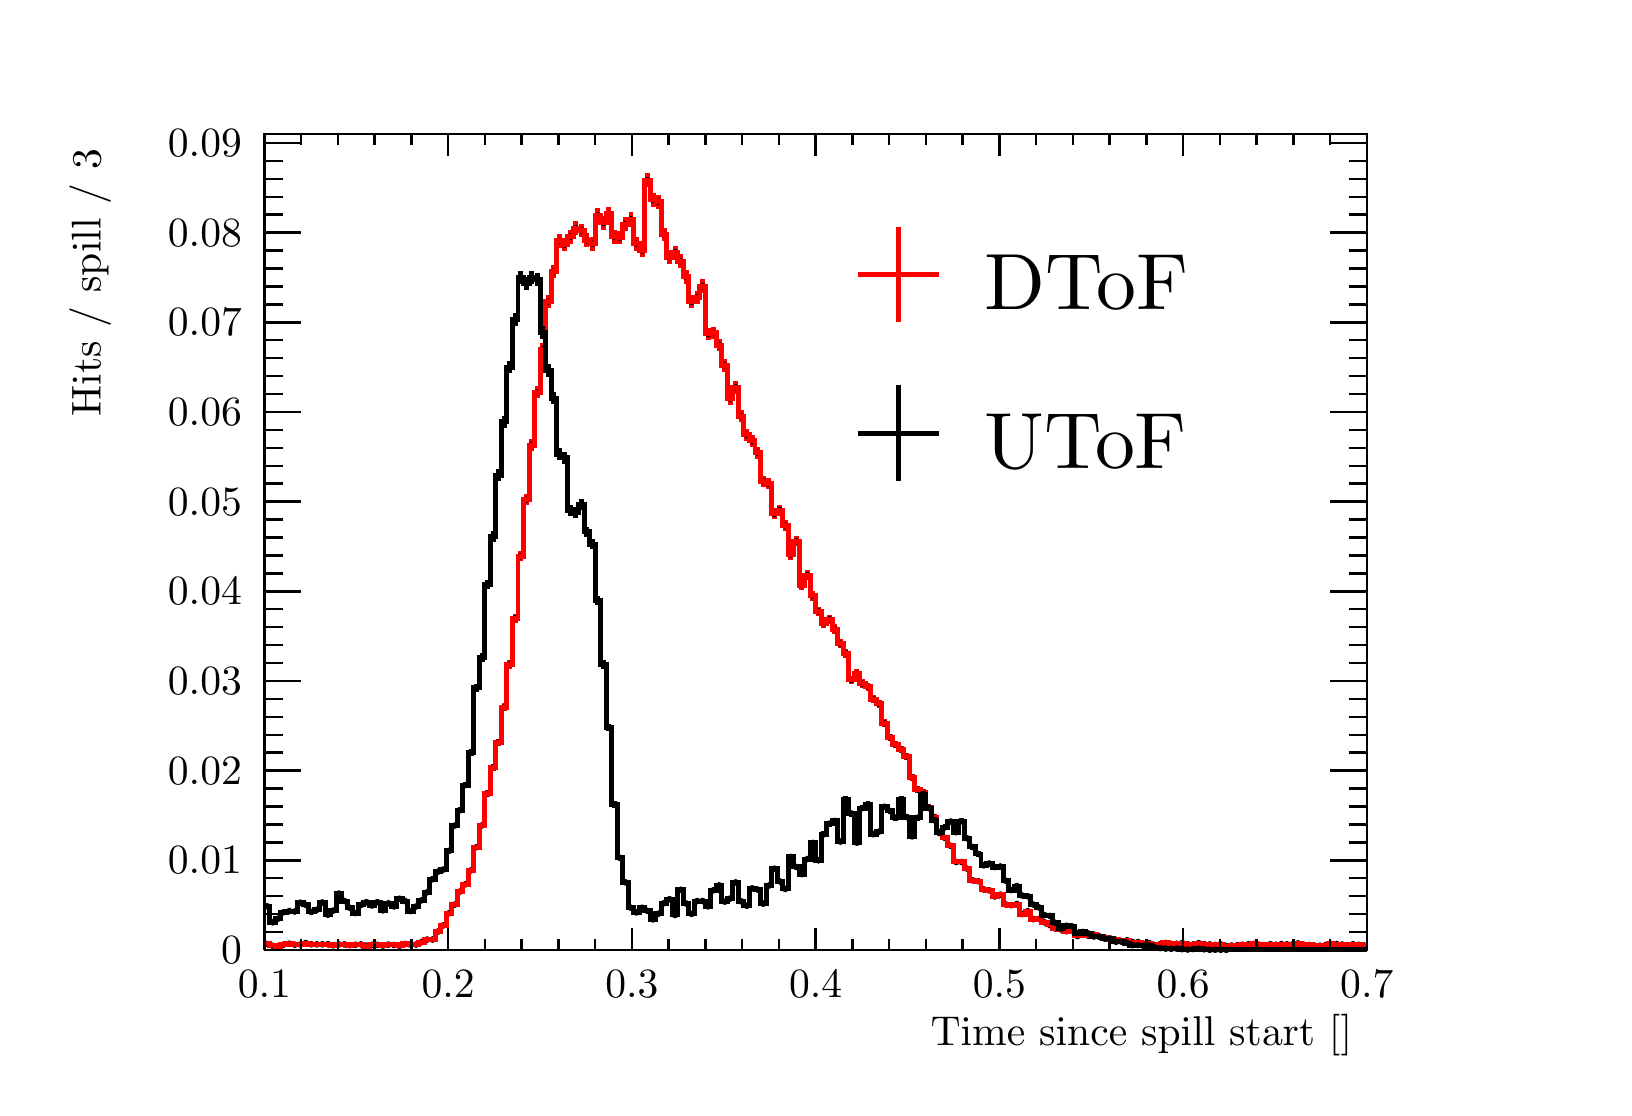
\begin{tikzpicture}
\pgfdeclareplotmark{cross} {
\pgfpathmoveto{\pgfpoint{-0.3\pgfplotmarksize}{\pgfplotmarksize}}
\pgfpathlineto{\pgfpoint{+0.3\pgfplotmarksize}{\pgfplotmarksize}}
\pgfpathlineto{\pgfpoint{+0.3\pgfplotmarksize}{0.3\pgfplotmarksize}}
\pgfpathlineto{\pgfpoint{+1\pgfplotmarksize}{0.3\pgfplotmarksize}}
\pgfpathlineto{\pgfpoint{+1\pgfplotmarksize}{-0.3\pgfplotmarksize}}
\pgfpathlineto{\pgfpoint{+0.3\pgfplotmarksize}{-0.3\pgfplotmarksize}}
\pgfpathlineto{\pgfpoint{+0.3\pgfplotmarksize}{-1.\pgfplotmarksize}}
\pgfpathlineto{\pgfpoint{-0.3\pgfplotmarksize}{-1.\pgfplotmarksize}}
\pgfpathlineto{\pgfpoint{-0.3\pgfplotmarksize}{-0.3\pgfplotmarksize}}
\pgfpathlineto{\pgfpoint{-1.\pgfplotmarksize}{-0.3\pgfplotmarksize}}
\pgfpathlineto{\pgfpoint{-1.\pgfplotmarksize}{0.3\pgfplotmarksize}}
\pgfpathlineto{\pgfpoint{-0.3\pgfplotmarksize}{0.3\pgfplotmarksize}}
\pgfpathclose
\pgfusepathqstroke
}
\pgfdeclareplotmark{cross*} {
\pgfpathmoveto{\pgfpoint{-0.3\pgfplotmarksize}{\pgfplotmarksize}}
\pgfpathlineto{\pgfpoint{+0.3\pgfplotmarksize}{\pgfplotmarksize}}
\pgfpathlineto{\pgfpoint{+0.3\pgfplotmarksize}{0.3\pgfplotmarksize}}
\pgfpathlineto{\pgfpoint{+1\pgfplotmarksize}{0.3\pgfplotmarksize}}
\pgfpathlineto{\pgfpoint{+1\pgfplotmarksize}{-0.3\pgfplotmarksize}}
\pgfpathlineto{\pgfpoint{+0.3\pgfplotmarksize}{-0.3\pgfplotmarksize}}
\pgfpathlineto{\pgfpoint{+0.3\pgfplotmarksize}{-1.\pgfplotmarksize}}
\pgfpathlineto{\pgfpoint{-0.3\pgfplotmarksize}{-1.\pgfplotmarksize}}
\pgfpathlineto{\pgfpoint{-0.3\pgfplotmarksize}{-0.3\pgfplotmarksize}}
\pgfpathlineto{\pgfpoint{-1.\pgfplotmarksize}{-0.3\pgfplotmarksize}}
\pgfpathlineto{\pgfpoint{-1.\pgfplotmarksize}{0.3\pgfplotmarksize}}
\pgfpathlineto{\pgfpoint{-0.3\pgfplotmarksize}{0.3\pgfplotmarksize}}
\pgfpathclose
\pgfusepathqfillstroke
}
\pgfdeclareplotmark{newstar} {
\pgfpathmoveto{\pgfqpoint{0pt}{\pgfplotmarksize}}
\pgfpathlineto{\pgfqpointpolar{44}{0.5\pgfplotmarksize}}
\pgfpathlineto{\pgfqpointpolar{18}{\pgfplotmarksize}}
\pgfpathlineto{\pgfqpointpolar{-20}{0.5\pgfplotmarksize}}
\pgfpathlineto{\pgfqpointpolar{-54}{\pgfplotmarksize}}
\pgfpathlineto{\pgfqpointpolar{-90}{0.5\pgfplotmarksize}}
\pgfpathlineto{\pgfqpointpolar{234}{\pgfplotmarksize}}
\pgfpathlineto{\pgfqpointpolar{198}{0.5\pgfplotmarksize}}
\pgfpathlineto{\pgfqpointpolar{162}{\pgfplotmarksize}}
\pgfpathlineto{\pgfqpointpolar{134}{0.5\pgfplotmarksize}}
\pgfpathclose
\pgfusepathqstroke
}
\pgfdeclareplotmark{newstar*} {
\pgfpathmoveto{\pgfqpoint{0pt}{\pgfplotmarksize}}
\pgfpathlineto{\pgfqpointpolar{44}{0.5\pgfplotmarksize}}
\pgfpathlineto{\pgfqpointpolar{18}{\pgfplotmarksize}}
\pgfpathlineto{\pgfqpointpolar{-20}{0.5\pgfplotmarksize}}
\pgfpathlineto{\pgfqpointpolar{-54}{\pgfplotmarksize}}
\pgfpathlineto{\pgfqpointpolar{-90}{0.5\pgfplotmarksize}}
\pgfpathlineto{\pgfqpointpolar{234}{\pgfplotmarksize}}
\pgfpathlineto{\pgfqpointpolar{198}{0.5\pgfplotmarksize}}
\pgfpathlineto{\pgfqpointpolar{162}{\pgfplotmarksize}}
\pgfpathlineto{\pgfqpointpolar{134}{0.5\pgfplotmarksize}}
\pgfpathclose
\pgfusepathqfillstroke
}
\definecolor{c}{rgb}{1,1,1};
\draw [color=c, fill=c] (0,0) rectangle (20,13.4556);
\draw [color=c, fill=c] (3,1.74922) rectangle (17,12.11);
\definecolor{c}{rgb}{0,0,0};
\draw [c,line width=0.9] (3,1.74922) -- (3,12.11) -- (17,12.11) -- (17,1.74922) -- (3,1.74922);
\definecolor{c}{rgb}{1,1,1};
\draw [color=c, fill=c] (3,1.74922) rectangle (17,12.11);
\definecolor{c}{rgb}{0,0,0};
\draw [c,line width=0.9] (3,1.74922) -- (3,12.11) -- (17,12.11) -- (17,1.74922) -- (3,1.74922);
\definecolor{c}{rgb}{1,0,0};
\draw [c,line width=1.8] (3.035,1.81776) -- (3.035,1.82578);
\draw [c,line width=1.8] (3.035,1.82578) -- (3.035,1.83381);
\definecolor{c}{rgb}{0,0,0};
\foreach \P in {(3.035,1.82578)}{\draw[mark options={color=c,fill=c},mark size=2.402402pt,mark=*,mark size=1pt] plot coordinates {\P};}
\definecolor{c}{rgb}{1,0,0};
\draw [c,line width=1.8] (3.105,1.79555) -- (3.105,1.80223);
\draw [c,line width=1.8] (3.105,1.80223) -- (3.105,1.8089);
\definecolor{c}{rgb}{0,0,0};
\foreach \P in {(3.105,1.80223)}{\draw[mark options={color=c,fill=c},mark size=2.402402pt,mark=*,mark size=1pt] plot coordinates {\P};}
\definecolor{c}{rgb}{1,0,0};
\draw [c,line width=1.8] (3.175,1.78691) -- (3.175,1.79297);
\draw [c,line width=1.8] (3.175,1.79297) -- (3.175,1.79904);
\definecolor{c}{rgb}{0,0,0};
\foreach \P in {(3.175,1.79297)}{\draw[mark options={color=c,fill=c},mark size=2.402402pt,mark=*,mark size=1pt] plot coordinates {\P};}
\definecolor{c}{rgb}{1,0,0};
\draw [c,line width=1.8] (3.245,1.81059) -- (3.245,1.81821);
\draw [c,line width=1.8] (3.245,1.81821) -- (3.245,1.82583);
\definecolor{c}{rgb}{0,0,0};
\foreach \P in {(3.245,1.81821)}{\draw[mark options={color=c,fill=c},mark size=2.402402pt,mark=*,mark size=1pt] plot coordinates {\P};}
\definecolor{c}{rgb}{1,0,0};
\draw [c,line width=1.8] (3.315,1.82095) -- (3.315,1.82915);
\draw [c,line width=1.8] (3.315,1.82915) -- (3.315,1.83735);
\definecolor{c}{rgb}{0,0,0};
\foreach \P in {(3.315,1.82915)}{\draw[mark options={color=c,fill=c},mark size=2.402402pt,mark=*,mark size=1pt] plot coordinates {\P};}
\definecolor{c}{rgb}{1,0,0};
\draw [c,line width=1.8] (3.385,1.809) -- (3.385,1.81653);
\draw [c,line width=1.8] (3.385,1.81653) -- (3.385,1.82405);
\definecolor{c}{rgb}{0,0,0};
\foreach \P in {(3.385,1.81653)}{\draw[mark options={color=c,fill=c},mark size=2.402402pt,mark=*,mark size=1pt] plot coordinates {\P};}
\definecolor{c}{rgb}{1,0,0};
\draw [c,line width=1.8] (3.455,1.81059) -- (3.455,1.81821);
\draw [c,line width=1.8] (3.455,1.81821) -- (3.455,1.82583);
\definecolor{c}{rgb}{0,0,0};
\foreach \P in {(3.455,1.81821)}{\draw[mark options={color=c,fill=c},mark size=2.402402pt,mark=*,mark size=1pt] plot coordinates {\P};}
\definecolor{c}{rgb}{1,0,0};
\draw [c,line width=1.8] (3.525,1.82814) -- (3.525,1.83672);
\draw [c,line width=1.8] (3.525,1.83672) -- (3.525,1.8453);
\definecolor{c}{rgb}{0,0,0};
\foreach \P in {(3.525,1.83672)}{\draw[mark options={color=c,fill=c},mark size=2.402402pt,mark=*,mark size=1pt] plot coordinates {\P};}
\definecolor{c}{rgb}{1,0,0};
\draw [c,line width=1.8] (3.595,1.81377) -- (3.595,1.82158);
\draw [c,line width=1.8] (3.595,1.82158) -- (3.595,1.82938);
\definecolor{c}{rgb}{0,0,0};
\foreach \P in {(3.595,1.82158)}{\draw[mark options={color=c,fill=c},mark size=2.402402pt,mark=*,mark size=1pt] plot coordinates {\P};}
\definecolor{c}{rgb}{1,0,0};
\draw [c,line width=1.8] (3.665,1.81298) -- (3.665,1.82073);
\draw [c,line width=1.8] (3.665,1.82073) -- (3.665,1.82849);
\definecolor{c}{rgb}{0,0,0};
\foreach \P in {(3.665,1.82073)}{\draw[mark options={color=c,fill=c},mark size=2.402402pt,mark=*,mark size=1pt] plot coordinates {\P};}
\definecolor{c}{rgb}{1,0,0};
\draw [c,line width=1.8] (3.735,1.81377) -- (3.735,1.82158);
\draw [c,line width=1.8] (3.735,1.82158) -- (3.735,1.82938);
\definecolor{c}{rgb}{0,0,0};
\foreach \P in {(3.735,1.82158)}{\draw[mark options={color=c,fill=c},mark size=2.402402pt,mark=*,mark size=1pt] plot coordinates {\P};}
\definecolor{c}{rgb}{1,0,0};
\draw [c,line width=1.8] (3.805,1.81457) -- (3.805,1.82242);
\draw [c,line width=1.8] (3.805,1.82242) -- (3.805,1.83026);
\definecolor{c}{rgb}{0,0,0};
\foreach \P in {(3.805,1.82242)}{\draw[mark options={color=c,fill=c},mark size=2.402402pt,mark=*,mark size=1pt] plot coordinates {\P};}
\definecolor{c}{rgb}{1,0,0};
\draw [c,line width=1.8] (3.875,1.80108) -- (3.875,1.80812);
\draw [c,line width=1.8] (3.875,1.80812) -- (3.875,1.81515);
\definecolor{c}{rgb}{0,0,0};
\foreach \P in {(3.875,1.80812)}{\draw[mark options={color=c,fill=c},mark size=2.402402pt,mark=*,mark size=1pt] plot coordinates {\P};}
\definecolor{c}{rgb}{1,0,0};
\draw [c,line width=1.8] (3.945,1.81298) -- (3.945,1.82073);
\draw [c,line width=1.8] (3.945,1.82073) -- (3.945,1.82849);
\definecolor{c}{rgb}{0,0,0};
\foreach \P in {(3.945,1.82073)}{\draw[mark options={color=c,fill=c},mark size=2.402402pt,mark=*,mark size=1pt] plot coordinates {\P};}
\definecolor{c}{rgb}{1,0,0};
\draw [c,line width=1.8] (4.015,1.81218) -- (4.015,1.81989);
\draw [c,line width=1.8] (4.015,1.81989) -- (4.015,1.8276);
\definecolor{c}{rgb}{0,0,0};
\foreach \P in {(4.015,1.81989)}{\draw[mark options={color=c,fill=c},mark size=2.402402pt,mark=*,mark size=1pt] plot coordinates {\P};}
\definecolor{c}{rgb}{1,0,0};
\draw [c,line width=1.8] (4.085,1.80345) -- (4.085,1.81064);
\draw [c,line width=1.8] (4.085,1.81064) -- (4.085,1.81783);
\definecolor{c}{rgb}{0,0,0};
\foreach \P in {(4.085,1.81064)}{\draw[mark options={color=c,fill=c},mark size=2.402402pt,mark=*,mark size=1pt] plot coordinates {\P};}
\definecolor{c}{rgb}{1,0,0};
\draw [c,line width=1.8] (4.155,1.80821) -- (4.155,1.81569);
\draw [c,line width=1.8] (4.155,1.81569) -- (4.155,1.82316);
\definecolor{c}{rgb}{0,0,0};
\foreach \P in {(4.155,1.81569)}{\draw[mark options={color=c,fill=c},mark size=2.402402pt,mark=*,mark size=1pt] plot coordinates {\P};}
\definecolor{c}{rgb}{1,0,0};
\draw [c,line width=1.8] (4.225,1.81218) -- (4.225,1.81989);
\draw [c,line width=1.8] (4.225,1.81989) -- (4.225,1.8276);
\definecolor{c}{rgb}{0,0,0};
\foreach \P in {(4.225,1.81989)}{\draw[mark options={color=c,fill=c},mark size=2.402402pt,mark=*,mark size=1pt] plot coordinates {\P};}
\definecolor{c}{rgb}{1,0,0};
\draw [c,line width=1.8] (4.295,1.7924) -- (4.295,1.79886);
\draw [c,line width=1.8] (4.295,1.79886) -- (4.295,1.80532);
\definecolor{c}{rgb}{0,0,0};
\foreach \P in {(4.295,1.79886)}{\draw[mark options={color=c,fill=c},mark size=2.402402pt,mark=*,mark size=1pt] plot coordinates {\P};}
\definecolor{c}{rgb}{1,0,0};
\draw [c,line width=1.8] (4.365,1.80742) -- (4.365,1.81485);
\draw [c,line width=1.8] (4.365,1.81485) -- (4.365,1.82228);
\definecolor{c}{rgb}{0,0,0};
\foreach \P in {(4.365,1.81485)}{\draw[mark options={color=c,fill=c},mark size=2.402402pt,mark=*,mark size=1pt] plot coordinates {\P};}
\definecolor{c}{rgb}{1,0,0};
\draw [c,line width=1.8] (4.435,1.80821) -- (4.435,1.81569);
\draw [c,line width=1.8] (4.435,1.81569) -- (4.435,1.82316);
\definecolor{c}{rgb}{0,0,0};
\foreach \P in {(4.435,1.81569)}{\draw[mark options={color=c,fill=c},mark size=2.402402pt,mark=*,mark size=1pt] plot coordinates {\P};}
\definecolor{c}{rgb}{1,0,0};
\draw [c,line width=1.8] (4.505,1.79792) -- (4.505,1.80475);
\draw [c,line width=1.8] (4.505,1.80475) -- (4.505,1.81158);
\definecolor{c}{rgb}{0,0,0};
\foreach \P in {(4.505,1.80475)}{\draw[mark options={color=c,fill=c},mark size=2.402402pt,mark=*,mark size=1pt] plot coordinates {\P};}
\definecolor{c}{rgb}{1,0,0};
\draw [c,line width=1.8] (4.575,1.8098) -- (4.575,1.81737);
\draw [c,line width=1.8] (4.575,1.81737) -- (4.575,1.82494);
\definecolor{c}{rgb}{0,0,0};
\foreach \P in {(4.575,1.81737)}{\draw[mark options={color=c,fill=c},mark size=2.402402pt,mark=*,mark size=1pt] plot coordinates {\P};}
\definecolor{c}{rgb}{1,0,0};
\draw [c,line width=1.8] (4.645,1.80583) -- (4.645,1.81316);
\draw [c,line width=1.8] (4.645,1.81316) -- (4.645,1.8205);
\definecolor{c}{rgb}{0,0,0};
\foreach \P in {(4.645,1.81316)}{\draw[mark options={color=c,fill=c},mark size=2.402402pt,mark=*,mark size=1pt] plot coordinates {\P};}
\definecolor{c}{rgb}{1,0,0};
\draw [c,line width=1.8] (4.715,1.79634) -- (4.715,1.80307);
\draw [c,line width=1.8] (4.715,1.80307) -- (4.715,1.8098);
\definecolor{c}{rgb}{0,0,0};
\foreach \P in {(4.715,1.80307)}{\draw[mark options={color=c,fill=c},mark size=2.402402pt,mark=*,mark size=1pt] plot coordinates {\P};}
\definecolor{c}{rgb}{1,0,0};
\draw [c,line width=1.8] (4.785,1.81776) -- (4.785,1.82578);
\draw [c,line width=1.8] (4.785,1.82578) -- (4.785,1.83381);
\definecolor{c}{rgb}{0,0,0};
\foreach \P in {(4.785,1.82578)}{\draw[mark options={color=c,fill=c},mark size=2.402402pt,mark=*,mark size=1pt] plot coordinates {\P};}
\definecolor{c}{rgb}{1,0,0};
\draw [c,line width=1.8] (4.855,1.8098) -- (4.855,1.81737);
\draw [c,line width=1.8] (4.855,1.81737) -- (4.855,1.82494);
\definecolor{c}{rgb}{0,0,0};
\foreach \P in {(4.855,1.81737)}{\draw[mark options={color=c,fill=c},mark size=2.402402pt,mark=*,mark size=1pt] plot coordinates {\P};}
\definecolor{c}{rgb}{1,0,0};
\draw [c,line width=1.8] (4.925,1.81059) -- (4.925,1.81821);
\draw [c,line width=1.8] (4.925,1.81821) -- (4.925,1.82583);
\definecolor{c}{rgb}{0,0,0};
\foreach \P in {(4.925,1.81821)}{\draw[mark options={color=c,fill=c},mark size=2.402402pt,mark=*,mark size=1pt] plot coordinates {\P};}
\definecolor{c}{rgb}{1,0,0};
\draw [c,line width=1.8] (4.995,1.83856) -- (4.995,1.84766);
\draw [c,line width=1.8] (4.995,1.84766) -- (4.995,1.85676);
\definecolor{c}{rgb}{0,0,0};
\foreach \P in {(4.995,1.84766)}{\draw[mark options={color=c,fill=c},mark size=2.402402pt,mark=*,mark size=1pt] plot coordinates {\P};}
\definecolor{c}{rgb}{1,0,0};
\draw [c,line width=1.8] (5.065,1.87077) -- (5.065,1.88131);
\draw [c,line width=1.8] (5.065,1.88131) -- (5.065,1.89185);
\definecolor{c}{rgb}{0,0,0};
\foreach \P in {(5.065,1.88131)}{\draw[mark options={color=c,fill=c},mark size=2.402402pt,mark=*,mark size=1pt] plot coordinates {\P};}
\definecolor{c}{rgb}{1,0,0};
\draw [c,line width=1.8] (5.135,1.87157) -- (5.135,1.88215);
\draw [c,line width=1.8] (5.135,1.88215) -- (5.135,1.89272);
\definecolor{c}{rgb}{0,0,0};
\foreach \P in {(5.135,1.88215)}{\draw[mark options={color=c,fill=c},mark size=2.402402pt,mark=*,mark size=1pt] plot coordinates {\P};}
\definecolor{c}{rgb}{1,0,0};
\draw [c,line width=1.8] (5.205,1.96989) -- (5.205,1.98395);
\draw [c,line width=1.8] (5.205,1.98395) -- (5.205,1.998);
\definecolor{c}{rgb}{0,0,0};
\foreach \P in {(5.205,1.98395)}{\draw[mark options={color=c,fill=c},mark size=2.402402pt,mark=*,mark size=1pt] plot coordinates {\P};}
\definecolor{c}{rgb}{1,0,0};
\draw [c,line width=1.8] (5.275,2.04596) -- (5.275,2.06219);
\draw [c,line width=1.8] (5.275,2.06219) -- (5.275,2.07841);
\definecolor{c}{rgb}{0,0,0};
\foreach \P in {(5.275,2.06219)}{\draw[mark options={color=c,fill=c},mark size=2.402402pt,mark=*,mark size=1pt] plot coordinates {\P};}
\definecolor{c}{rgb}{1,0,0};
\draw [c,line width=1.8] (5.345,2.19633) -- (5.345,2.21614);
\draw [c,line width=1.8] (5.345,2.21614) -- (5.345,2.23596);
\definecolor{c}{rgb}{0,0,0};
\foreach \P in {(5.345,2.21614)}{\draw[mark options={color=c,fill=c},mark size=2.402402pt,mark=*,mark size=1pt] plot coordinates {\P};}
\definecolor{c}{rgb}{1,0,0};
\draw [c,line width=1.8] (5.415,2.30349) -- (5.415,2.32551);
\draw [c,line width=1.8] (5.415,2.32551) -- (5.415,2.34753);
\definecolor{c}{rgb}{0,0,0};
\foreach \P in {(5.415,2.32551)}{\draw[mark options={color=c,fill=c},mark size=2.402402pt,mark=*,mark size=1pt] plot coordinates {\P};}
\definecolor{c}{rgb}{1,0,0};
\draw [c,line width=1.8] (5.485,2.46709) -- (5.485,2.49209);
\draw [c,line width=1.8] (5.485,2.49209) -- (5.485,2.51709);
\definecolor{c}{rgb}{0,0,0};
\foreach \P in {(5.485,2.49209)}{\draw[mark options={color=c,fill=c},mark size=2.402402pt,mark=*,mark size=1pt] plot coordinates {\P};}
\definecolor{c}{rgb}{1,0,0};
\draw [c,line width=1.8] (5.555,2.55812) -- (5.555,2.58463);
\draw [c,line width=1.8] (5.555,2.58463) -- (5.555,2.61114);
\definecolor{c}{rgb}{0,0,0};
\foreach \P in {(5.555,2.58463)}{\draw[mark options={color=c,fill=c},mark size=2.402402pt,mark=*,mark size=1pt] plot coordinates {\P};}
\definecolor{c}{rgb}{1,0,0};
\draw [c,line width=1.8] (5.625,2.73213) -- (5.625,2.76131);
\draw [c,line width=1.8] (5.625,2.76131) -- (5.625,2.79049);
\definecolor{c}{rgb}{0,0,0};
\foreach \P in {(5.625,2.76131)}{\draw[mark options={color=c,fill=c},mark size=2.402402pt,mark=*,mark size=1pt] plot coordinates {\P};}
\definecolor{c}{rgb}{1,0,0};
\draw [c,line width=1.8] (5.695,3.02178) -- (5.695,3.05492);
\draw [c,line width=1.8] (5.695,3.05492) -- (5.695,3.08806);
\definecolor{c}{rgb}{0,0,0};
\foreach \P in {(5.695,3.05492)}{\draw[mark options={color=c,fill=c},mark size=2.402402pt,mark=*,mark size=1pt] plot coordinates {\P};}
\definecolor{c}{rgb}{1,0,0};
\draw [c,line width=1.8] (5.765,3.29522) -- (5.765,3.33171);
\draw [c,line width=1.8] (5.765,3.33171) -- (5.765,3.36819);
\definecolor{c}{rgb}{0,0,0};
\foreach \P in {(5.765,3.33171)}{\draw[mark options={color=c,fill=c},mark size=2.402402pt,mark=*,mark size=1pt] plot coordinates {\P};}
\definecolor{c}{rgb}{1,0,0};
\draw [c,line width=1.8] (5.835,3.69715) -- (5.835,3.73805);
\draw [c,line width=1.8] (5.835,3.73805) -- (5.835,3.77896);
\definecolor{c}{rgb}{0,0,0};
\foreach \P in {(5.835,3.73805)}{\draw[mark options={color=c,fill=c},mark size=2.402402pt,mark=*,mark size=1pt] plot coordinates {\P};}
\definecolor{c}{rgb}{1,0,0};
\draw [c,line width=1.8] (5.905,4.02618) -- (5.905,4.07037);
\draw [c,line width=1.8] (5.905,4.07037) -- (5.905,4.11456);
\definecolor{c}{rgb}{0,0,0};
\foreach \P in {(5.905,4.07037)}{\draw[mark options={color=c,fill=c},mark size=2.402402pt,mark=*,mark size=1pt] plot coordinates {\P};}
\definecolor{c}{rgb}{1,0,0};
\draw [c,line width=1.8] (5.975,4.33959) -- (5.975,4.38669);
\draw [c,line width=1.8] (5.975,4.38669) -- (5.975,4.4338);
\definecolor{c}{rgb}{0,0,0};
\foreach \P in {(5.975,4.38669)}{\draw[mark options={color=c,fill=c},mark size=2.402402pt,mark=*,mark size=1pt] plot coordinates {\P};}
\definecolor{c}{rgb}{1,0,0};
\draw [c,line width=1.8] (6.045,4.78249) -- (6.045,4.83342);
\draw [c,line width=1.8] (6.045,4.83342) -- (6.045,4.88436);
\definecolor{c}{rgb}{0,0,0};
\foreach \P in {(6.045,4.83342)}{\draw[mark options={color=c,fill=c},mark size=2.402402pt,mark=*,mark size=1pt] plot coordinates {\P};}
\definecolor{c}{rgb}{1,0,0};
\draw [c,line width=1.8] (6.115,5.32166) -- (6.115,5.3769);
\draw [c,line width=1.8] (6.115,5.3769) -- (6.115,5.43215);
\definecolor{c}{rgb}{0,0,0};
\foreach \P in {(6.115,5.3769)}{\draw[mark options={color=c,fill=c},mark size=2.402402pt,mark=*,mark size=1pt] plot coordinates {\P};}
\definecolor{c}{rgb}{1,0,0};
\draw [c,line width=1.8] (6.185,5.90291) -- (6.185,5.96245);
\draw [c,line width=1.8] (6.185,5.96245) -- (6.185,6.02198);
\definecolor{c}{rgb}{0,0,0};
\foreach \P in {(6.185,5.96245)}{\draw[mark options={color=c,fill=c},mark size=2.402402pt,mark=*,mark size=1pt] plot coordinates {\P};}
\definecolor{c}{rgb}{1,0,0};
\draw [c,line width=1.8] (6.255,6.68504) -- (6.255,6.7499);
\draw [c,line width=1.8] (6.255,6.7499) -- (6.255,6.81476);
\definecolor{c}{rgb}{0,0,0};
\foreach \P in {(6.255,6.7499)}{\draw[mark options={color=c,fill=c},mark size=2.402402pt,mark=*,mark size=1pt] plot coordinates {\P};}
\definecolor{c}{rgb}{1,0,0};
\draw [c,line width=1.8] (6.325,7.39817) -- (6.325,7.46753);
\draw [c,line width=1.8] (6.325,7.46753) -- (6.325,7.53689);
\definecolor{c}{rgb}{0,0,0};
\foreach \P in {(6.325,7.46753)}{\draw[mark options={color=c,fill=c},mark size=2.402402pt,mark=*,mark size=1pt] plot coordinates {\P};}
\definecolor{c}{rgb}{1,0,0};
\draw [c,line width=1.8] (6.395,8.08815) -- (6.395,8.1616);
\draw [c,line width=1.8] (6.395,8.1616) -- (6.395,8.23505);
\definecolor{c}{rgb}{0,0,0};
\foreach \P in {(6.395,8.1616)}{\draw[mark options={color=c,fill=c},mark size=2.402402pt,mark=*,mark size=1pt] plot coordinates {\P};}
\definecolor{c}{rgb}{1,0,0};
\draw [c,line width=1.8] (6.465,8.75408) -- (6.465,8.83127);
\draw [c,line width=1.8] (6.465,8.83127) -- (6.465,8.90846);
\definecolor{c}{rgb}{0,0,0};
\foreach \P in {(6.465,8.83127)}{\draw[mark options={color=c,fill=c},mark size=2.402402pt,mark=*,mark size=1pt] plot coordinates {\P};}
\definecolor{c}{rgb}{1,0,0};
\draw [c,line width=1.8] (6.535,9.30051) -- (6.535,9.38064);
\draw [c,line width=1.8] (6.535,9.38064) -- (6.535,9.46077);
\definecolor{c}{rgb}{0,0,0};
\foreach \P in {(6.535,9.38064)}{\draw[mark options={color=c,fill=c},mark size=2.402402pt,mark=*,mark size=1pt] plot coordinates {\P};}
\definecolor{c}{rgb}{1,0,0};
\draw [c,line width=1.8] (6.605,9.90229) -- (6.605,9.98553);
\draw [c,line width=1.8] (6.605,9.98553) -- (6.605,10.0688);
\definecolor{c}{rgb}{0,0,0};
\foreach \P in {(6.605,9.98553)}{\draw[mark options={color=c,fill=c},mark size=2.402402pt,mark=*,mark size=1pt] plot coordinates {\P};}
\definecolor{c}{rgb}{1,0,0};
\draw [c,line width=1.8] (6.675,10.2815) -- (6.675,10.3666);
\draw [c,line width=1.8] (6.675,10.3666) -- (6.675,10.4518);
\definecolor{c}{rgb}{0,0,0};
\foreach \P in {(6.675,10.3666)}{\draw[mark options={color=c,fill=c},mark size=2.402402pt,mark=*,mark size=1pt] plot coordinates {\P};}
\definecolor{c}{rgb}{1,0,0};
\draw [c,line width=1.8] (6.745,10.6674) -- (6.745,10.7545);
\draw [c,line width=1.8] (6.745,10.7545) -- (6.745,10.8415);
\definecolor{c}{rgb}{0,0,0};
\foreach \P in {(6.745,10.7545)}{\draw[mark options={color=c,fill=c},mark size=2.402402pt,mark=*,mark size=1pt] plot coordinates {\P};}
\definecolor{c}{rgb}{1,0,0};
\draw [c,line width=1.8] (6.815,10.6206) -- (6.815,10.7074);
\draw [c,line width=1.8] (6.815,10.7074) -- (6.815,10.7942);
\definecolor{c}{rgb}{0,0,0};
\foreach \P in {(6.815,10.7074)}{\draw[mark options={color=c,fill=c},mark size=2.402402pt,mark=*,mark size=1pt] plot coordinates {\P};}
\definecolor{c}{rgb}{1,0,0};
\draw [c,line width=1.8] (6.885,10.721) -- (6.885,10.8083);
\draw [c,line width=1.8] (6.885,10.8083) -- (6.885,10.8956);
\definecolor{c}{rgb}{0,0,0};
\foreach \P in {(6.885,10.8083)}{\draw[mark options={color=c,fill=c},mark size=2.402402pt,mark=*,mark size=1pt] plot coordinates {\P};}
\definecolor{c}{rgb}{1,0,0};
\draw [c,line width=1.8] (6.955,10.8282) -- (6.955,10.916);
\draw [c,line width=1.8] (6.955,10.916) -- (6.955,11.0038);
\definecolor{c}{rgb}{0,0,0};
\foreach \P in {(6.955,10.916)}{\draw[mark options={color=c,fill=c},mark size=2.402402pt,mark=*,mark size=1pt] plot coordinates {\P};}
\definecolor{c}{rgb}{1,0,0};
\draw [c,line width=1.8] (7.025,10.7997) -- (7.025,10.8874);
\draw [c,line width=1.8] (7.025,10.8874) -- (7.025,10.9751);
\definecolor{c}{rgb}{0,0,0};
\foreach \P in {(7.025,10.8874)}{\draw[mark options={color=c,fill=c},mark size=2.402402pt,mark=*,mark size=1pt] plot coordinates {\P};}
\definecolor{c}{rgb}{1,0,0};
\draw [c,line width=1.8] (7.095,10.6758) -- (7.095,10.7629);
\draw [c,line width=1.8] (7.095,10.7629) -- (7.095,10.85);
\definecolor{c}{rgb}{0,0,0};
\foreach \P in {(7.095,10.7629)}{\draw[mark options={color=c,fill=c},mark size=2.402402pt,mark=*,mark size=1pt] plot coordinates {\P};}
\definecolor{c}{rgb}{1,0,0};
\draw [c,line width=1.8] (7.165,10.6314) -- (7.165,10.7183);
\draw [c,line width=1.8] (7.165,10.7183) -- (7.165,10.8052);
\definecolor{c}{rgb}{0,0,0};
\foreach \P in {(7.165,10.7183)}{\draw[mark options={color=c,fill=c},mark size=2.402402pt,mark=*,mark size=1pt] plot coordinates {\P};}
\definecolor{c}{rgb}{1,0,0};
\draw [c,line width=1.8] (7.235,10.9898) -- (7.235,11.0784);
\draw [c,line width=1.8] (7.235,11.0784) -- (7.235,11.167);
\definecolor{c}{rgb}{0,0,0};
\foreach \P in {(7.235,11.0784)}{\draw[mark options={color=c,fill=c},mark size=2.402402pt,mark=*,mark size=1pt] plot coordinates {\P};}
\definecolor{c}{rgb}{1,0,0};
\draw [c,line width=1.8] (7.305,10.896) -- (7.305,10.9842);
\draw [c,line width=1.8] (7.305,10.9842) -- (7.305,11.0723);
\definecolor{c}{rgb}{0,0,0};
\foreach \P in {(7.305,10.9842)}{\draw[mark options={color=c,fill=c},mark size=2.402402pt,mark=*,mark size=1pt] plot coordinates {\P};}
\definecolor{c}{rgb}{1,0,0};
\draw [c,line width=1.8] (7.375,11.0107) -- (7.375,11.0994);
\draw [c,line width=1.8] (7.375,11.0994) -- (7.375,11.1881);
\definecolor{c}{rgb}{0,0,0};
\foreach \P in {(7.375,11.0994)}{\draw[mark options={color=c,fill=c},mark size=2.402402pt,mark=*,mark size=1pt] plot coordinates {\P};}
\definecolor{c}{rgb}{1,0,0};
\draw [c,line width=1.8] (7.445,10.7193) -- (7.445,10.8066);
\draw [c,line width=1.8] (7.445,10.8066) -- (7.445,10.8939);
\definecolor{c}{rgb}{0,0,0};
\foreach \P in {(7.445,10.8066)}{\draw[mark options={color=c,fill=c},mark size=2.402402pt,mark=*,mark size=1pt] plot coordinates {\P};}
\definecolor{c}{rgb}{1,0,0};
\draw [c,line width=1.8] (7.515,10.711) -- (7.515,10.7982);
\draw [c,line width=1.8] (7.515,10.7982) -- (7.515,10.8855);
\definecolor{c}{rgb}{0,0,0};
\foreach \P in {(7.515,10.7982)}{\draw[mark options={color=c,fill=c},mark size=2.402402pt,mark=*,mark size=1pt] plot coordinates {\P};}
\definecolor{c}{rgb}{1,0,0};
\draw [c,line width=1.8] (7.585,10.8801) -- (7.585,10.9682);
\draw [c,line width=1.8] (7.585,10.9682) -- (7.585,11.0562);
\definecolor{c}{rgb}{0,0,0};
\foreach \P in {(7.585,10.9682)}{\draw[mark options={color=c,fill=c},mark size=2.402402pt,mark=*,mark size=1pt] plot coordinates {\P};}
\definecolor{c}{rgb}{1,0,0};
\draw [c,line width=1.8] (7.655,10.9395) -- (7.655,11.0279);
\draw [c,line width=1.8] (7.655,11.0279) -- (7.655,11.1163);
\definecolor{c}{rgb}{0,0,0};
\foreach \P in {(7.655,11.0279)}{\draw[mark options={color=c,fill=c},mark size=2.402402pt,mark=*,mark size=1pt] plot coordinates {\P};}
\definecolor{c}{rgb}{1,0,0};
\draw [c,line width=1.8] (7.725,10.6323) -- (7.725,10.7191);
\draw [c,line width=1.8] (7.725,10.7191) -- (7.725,10.806);
\definecolor{c}{rgb}{0,0,0};
\foreach \P in {(7.725,10.7191)}{\draw[mark options={color=c,fill=c},mark size=2.402402pt,mark=*,mark size=1pt] plot coordinates {\P};}
\definecolor{c}{rgb}{1,0,0};
\draw [c,line width=1.8] (7.795,10.5452) -- (7.795,10.6317);
\draw [c,line width=1.8] (7.795,10.6317) -- (7.795,10.7181);
\definecolor{c}{rgb}{0,0,0};
\foreach \P in {(7.795,10.6317)}{\draw[mark options={color=c,fill=c},mark size=2.402402pt,mark=*,mark size=1pt] plot coordinates {\P};}
\definecolor{c}{rgb}{1,0,0};
\draw [c,line width=1.8] (7.865,11.4353) -- (7.865,11.526);
\draw [c,line width=1.8] (7.865,11.526) -- (7.865,11.6166);
\definecolor{c}{rgb}{0,0,0};
\foreach \P in {(7.865,11.526)}{\draw[mark options={color=c,fill=c},mark size=2.402402pt,mark=*,mark size=1pt] plot coordinates {\P};}
\definecolor{c}{rgb}{1,0,0};
\draw [c,line width=1.8] (7.935,11.1849) -- (7.935,11.2744);
\draw [c,line width=1.8] (7.935,11.2744) -- (7.935,11.3639);
\definecolor{c}{rgb}{0,0,0};
\foreach \P in {(7.935,11.2744)}{\draw[mark options={color=c,fill=c},mark size=2.402402pt,mark=*,mark size=1pt] plot coordinates {\P};}
\definecolor{c}{rgb}{1,0,0};
\draw [c,line width=1.8] (8.005,11.1598) -- (8.005,11.2492);
\draw [c,line width=1.8] (8.005,11.2492) -- (8.005,11.3386);
\definecolor{c}{rgb}{0,0,0};
\foreach \P in {(8.005,11.2492)}{\draw[mark options={color=c,fill=c},mark size=2.402402pt,mark=*,mark size=1pt] plot coordinates {\P};}
\definecolor{c}{rgb}{1,0,0};
\draw [c,line width=1.8] (8.075,10.747) -- (8.075,10.8344);
\draw [c,line width=1.8] (8.075,10.8344) -- (8.075,10.9218);
\definecolor{c}{rgb}{0,0,0};
\foreach \P in {(8.075,10.8344)}{\draw[mark options={color=c,fill=c},mark size=2.402402pt,mark=*,mark size=1pt] plot coordinates {\P};}
\definecolor{c}{rgb}{1,0,0};
\draw [c,line width=1.8] (8.145,10.4615) -- (8.145,10.5475);
\draw [c,line width=1.8] (8.145,10.5475) -- (8.145,10.6336);
\definecolor{c}{rgb}{0,0,0};
\foreach \P in {(8.145,10.5475)}{\draw[mark options={color=c,fill=c},mark size=2.402402pt,mark=*,mark size=1pt] plot coordinates {\P};}
\definecolor{c}{rgb}{1,0,0};
\draw [c,line width=1.8] (8.215,10.5226) -- (8.215,10.6089);
\draw [c,line width=1.8] (8.215,10.6089) -- (8.215,10.6953);
\definecolor{c}{rgb}{0,0,0};
\foreach \P in {(8.215,10.6089)}{\draw[mark options={color=c,fill=c},mark size=2.402402pt,mark=*,mark size=1pt] plot coordinates {\P};}
\definecolor{c}{rgb}{1,0,0};
\draw [c,line width=1.8] (8.285,10.4121) -- (8.285,10.4979);
\draw [c,line width=1.8] (8.285,10.4979) -- (8.285,10.5837);
\definecolor{c}{rgb}{0,0,0};
\foreach \P in {(8.285,10.4979)}{\draw[mark options={color=c,fill=c},mark size=2.402402pt,mark=*,mark size=1pt] plot coordinates {\P};}
\definecolor{c}{rgb}{1,0,0};
\draw [c,line width=1.8] (8.355,10.2129) -- (8.355,10.2977);
\draw [c,line width=1.8] (8.355,10.2977) -- (8.355,10.3825);
\definecolor{c}{rgb}{0,0,0};
\foreach \P in {(8.355,10.2977)}{\draw[mark options={color=c,fill=c},mark size=2.402402pt,mark=*,mark size=1pt] plot coordinates {\P};}
\definecolor{c}{rgb}{1,0,0};
\draw [c,line width=1.8] (8.425,9.89811) -- (8.425,9.98133);
\draw [c,line width=1.8] (8.425,9.98133) -- (8.425,10.0645);
\definecolor{c}{rgb}{0,0,0};
\foreach \P in {(8.425,9.98133)}{\draw[mark options={color=c,fill=c},mark size=2.402402pt,mark=*,mark size=1pt] plot coordinates {\P};}
\definecolor{c}{rgb}{1,0,0};
\draw [c,line width=1.8] (8.495,9.95503) -- (8.495,10.0385);
\draw [c,line width=1.8] (8.495,10.0385) -- (8.495,10.122);
\definecolor{c}{rgb}{0,0,0};
\foreach \P in {(8.495,10.0385)}{\draw[mark options={color=c,fill=c},mark size=2.402402pt,mark=*,mark size=1pt] plot coordinates {\P};}
\definecolor{c}{rgb}{1,0,0};
\draw [c,line width=1.8] (8.565,10.0965) -- (8.565,10.1807);
\draw [c,line width=1.8] (8.565,10.1807) -- (8.565,10.2649);
\definecolor{c}{rgb}{0,0,0};
\foreach \P in {(8.565,10.1807)}{\draw[mark options={color=c,fill=c},mark size=2.402402pt,mark=*,mark size=1pt] plot coordinates {\P};}
\definecolor{c}{rgb}{1,0,0};
\draw [c,line width=1.8] (8.635,9.49217) -- (8.635,9.5733);
\draw [c,line width=1.8] (8.635,9.5733) -- (8.635,9.65443);
\definecolor{c}{rgb}{0,0,0};
\foreach \P in {(8.635,9.5733)}{\draw[mark options={color=c,fill=c},mark size=2.402402pt,mark=*,mark size=1pt] plot coordinates {\P};}
\definecolor{c}{rgb}{1,0,0};
\draw [c,line width=1.8] (8.705,9.50388) -- (8.705,9.58508);
\draw [c,line width=1.8] (8.705,9.58508) -- (8.705,9.66627);
\definecolor{c}{rgb}{0,0,0};
\foreach \P in {(8.705,9.58508)}{\draw[mark options={color=c,fill=c},mark size=2.402402pt,mark=*,mark size=1pt] plot coordinates {\P};}
\definecolor{c}{rgb}{1,0,0};
\draw [c,line width=1.8] (8.775,9.35156) -- (8.775,9.43196);
\draw [c,line width=1.8] (8.775,9.43196) -- (8.775,9.51235);
\definecolor{c}{rgb}{0,0,0};
\foreach \P in {(8.775,9.43196)}{\draw[mark options={color=c,fill=c},mark size=2.402402pt,mark=*,mark size=1pt] plot coordinates {\P};}
\definecolor{c}{rgb}{1,0,0};
\draw [c,line width=1.8] (8.845,9.09381) -- (8.845,9.17284);
\draw [c,line width=1.8] (8.845,9.17284) -- (8.845,9.25187);
\definecolor{c}{rgb}{0,0,0};
\foreach \P in {(8.845,9.17284)}{\draw[mark options={color=c,fill=c},mark size=2.402402pt,mark=*,mark size=1pt] plot coordinates {\P};}
\definecolor{c}{rgb}{1,0,0};
\draw [c,line width=1.8] (8.915,8.67627) -- (8.915,8.75303);
\draw [c,line width=1.8] (8.915,8.75303) -- (8.915,8.82979);
\definecolor{c}{rgb}{0,0,0};
\foreach \P in {(8.915,8.75303)}{\draw[mark options={color=c,fill=c},mark size=2.402402pt,mark=*,mark size=1pt] plot coordinates {\P};}
\definecolor{c}{rgb}{1,0,0};
\draw [c,line width=1.8] (8.985,8.816) -- (8.985,8.89353);
\draw [c,line width=1.8] (8.985,8.89353) -- (8.985,8.97106);
\definecolor{c}{rgb}{0,0,0};
\foreach \P in {(8.985,8.89353)}{\draw[mark options={color=c,fill=c},mark size=2.402402pt,mark=*,mark size=1pt] plot coordinates {\P};}
\definecolor{c}{rgb}{1,0,0};
\draw [c,line width=1.8] (9.055,8.45121) -- (9.055,8.52672);
\draw [c,line width=1.8] (9.055,8.52672) -- (9.055,8.60223);
\definecolor{c}{rgb}{0,0,0};
\foreach \P in {(9.055,8.52672)}{\draw[mark options={color=c,fill=c},mark size=2.402402pt,mark=*,mark size=1pt] plot coordinates {\P};}
\definecolor{c}{rgb}{1,0,0};
\draw [c,line width=1.8] (9.125,8.21781) -- (9.125,8.292);
\draw [c,line width=1.8] (9.125,8.292) -- (9.125,8.36619);
\definecolor{c}{rgb}{0,0,0};
\foreach \P in {(9.125,8.292)}{\draw[mark options={color=c,fill=c},mark size=2.402402pt,mark=*,mark size=1pt] plot coordinates {\P};}
\definecolor{c}{rgb}{1,0,0};
\draw [c,line width=1.8] (9.195,8.14085) -- (9.195,8.2146);
\draw [c,line width=1.8] (9.195,8.2146) -- (9.195,8.28835);
\definecolor{c}{rgb}{0,0,0};
\foreach \P in {(9.195,8.2146)}{\draw[mark options={color=c,fill=c},mark size=2.402402pt,mark=*,mark size=1pt] plot coordinates {\P};}
\definecolor{c}{rgb}{1,0,0};
\draw [c,line width=1.8] (9.265,7.99028) -- (9.265,8.06317);
\draw [c,line width=1.8] (9.265,8.06317) -- (9.265,8.13605);
\definecolor{c}{rgb}{0,0,0};
\foreach \P in {(9.265,8.06317)}{\draw[mark options={color=c,fill=c},mark size=2.402402pt,mark=*,mark size=1pt] plot coordinates {\P};}
\definecolor{c}{rgb}{1,0,0};
\draw [c,line width=1.8] (9.335,7.63064) -- (9.335,7.70141);
\draw [c,line width=1.8] (9.335,7.70141) -- (9.335,7.77217);
\definecolor{c}{rgb}{0,0,0};
\foreach \P in {(9.335,7.70141)}{\draw[mark options={color=c,fill=c},mark size=2.402402pt,mark=*,mark size=1pt] plot coordinates {\P};}
\definecolor{c}{rgb}{1,0,0};
\draw [c,line width=1.8] (9.405,7.60054) -- (9.405,7.67112);
\draw [c,line width=1.8] (9.405,7.67112) -- (9.405,7.74171);
\definecolor{c}{rgb}{0,0,0};
\foreach \P in {(9.405,7.67112)}{\draw[mark options={color=c,fill=c},mark size=2.402402pt,mark=*,mark size=1pt] plot coordinates {\P};}
\definecolor{c}{rgb}{1,0,0};
\draw [c,line width=1.8] (9.475,7.2209) -- (9.475,7.28917);
\draw [c,line width=1.8] (9.475,7.28917) -- (9.475,7.35744);
\definecolor{c}{rgb}{0,0,0};
\foreach \P in {(9.475,7.28917)}{\draw[mark options={color=c,fill=c},mark size=2.402402pt,mark=*,mark size=1pt] plot coordinates {\P};}
\definecolor{c}{rgb}{1,0,0};
\draw [c,line width=1.8] (9.545,7.26773) -- (9.545,7.33629);
\draw [c,line width=1.8] (9.545,7.33629) -- (9.545,7.40484);
\definecolor{c}{rgb}{0,0,0};
\foreach \P in {(9.545,7.33629)}{\draw[mark options={color=c,fill=c},mark size=2.402402pt,mark=*,mark size=1pt] plot coordinates {\P};}
\definecolor{c}{rgb}{1,0,0};
\draw [c,line width=1.8] (9.615,7.07459) -- (9.615,7.14195);
\draw [c,line width=1.8] (9.615,7.14195) -- (9.615,7.2093);
\definecolor{c}{rgb}{0,0,0};
\foreach \P in {(9.615,7.14195)}{\draw[mark options={color=c,fill=c},mark size=2.402402pt,mark=*,mark size=1pt] plot coordinates {\P};}
\definecolor{c}{rgb}{1,0,0};
\draw [c,line width=1.8] (9.685,6.70594) -- (9.685,6.77093);
\draw [c,line width=1.8] (9.685,6.77093) -- (9.685,6.83593);
\definecolor{c}{rgb}{0,0,0};
\foreach \P in {(9.685,6.77093)}{\draw[mark options={color=c,fill=c},mark size=2.402402pt,mark=*,mark size=1pt] plot coordinates {\P};}
\definecolor{c}{rgb}{1,0,0};
\draw [c,line width=1.8] (9.755,6.87562) -- (9.755,6.94172);
\draw [c,line width=1.8] (9.755,6.94172) -- (9.755,7.00781);
\definecolor{c}{rgb}{0,0,0};
\foreach \P in {(9.755,6.94172)}{\draw[mark options={color=c,fill=c},mark size=2.402402pt,mark=*,mark size=1pt] plot coordinates {\P};}
\definecolor{c}{rgb}{1,0,0};
\draw [c,line width=1.8] (9.825,6.31982) -- (9.825,6.38225);
\draw [c,line width=1.8] (9.825,6.38225) -- (9.825,6.44469);
\definecolor{c}{rgb}{0,0,0};
\foreach \P in {(9.825,6.38225)}{\draw[mark options={color=c,fill=c},mark size=2.402402pt,mark=*,mark size=1pt] plot coordinates {\P};}
\definecolor{c}{rgb}{1,0,0};
\draw [c,line width=1.8] (9.895,6.44434) -- (9.895,6.50761);
\draw [c,line width=1.8] (9.895,6.50761) -- (9.895,6.57088);
\definecolor{c}{rgb}{0,0,0};
\foreach \P in {(9.895,6.50761)}{\draw[mark options={color=c,fill=c},mark size=2.402402pt,mark=*,mark size=1pt] plot coordinates {\P};}
\definecolor{c}{rgb}{1,0,0};
\draw [c,line width=1.8] (9.965,6.18529) -- (9.965,6.2468);
\draw [c,line width=1.8] (9.965,6.2468) -- (9.965,6.30832);
\definecolor{c}{rgb}{0,0,0};
\foreach \P in {(9.965,6.2468)}{\draw[mark options={color=c,fill=c},mark size=2.402402pt,mark=*,mark size=1pt] plot coordinates {\P};}
\definecolor{c}{rgb}{1,0,0};
\draw [c,line width=1.8] (10.035,5.99062) -- (10.035,6.05078);
\draw [c,line width=1.8] (10.035,6.05078) -- (10.035,6.11094);
\definecolor{c}{rgb}{0,0,0};
\foreach \P in {(10.035,6.05078)}{\draw[mark options={color=c,fill=c},mark size=2.402402pt,mark=*,mark size=1pt] plot coordinates {\P};}
\definecolor{c}{rgb}{1,0,0};
\draw [c,line width=1.8] (10.105,5.83942) -- (10.105,5.89851);
\draw [c,line width=1.8] (10.105,5.89851) -- (10.105,5.95759);
\definecolor{c}{rgb}{0,0,0};
\foreach \P in {(10.105,5.89851)}{\draw[mark options={color=c,fill=c},mark size=2.402402pt,mark=*,mark size=1pt] plot coordinates {\P};}
\definecolor{c}{rgb}{1,0,0};
\draw [c,line width=1.8] (10.175,5.88871) -- (10.175,5.94814);
\draw [c,line width=1.8] (10.175,5.94814) -- (10.175,6.00758);
\definecolor{c}{rgb}{0,0,0};
\foreach \P in {(10.175,5.94814)}{\draw[mark options={color=c,fill=c},mark size=2.402402pt,mark=*,mark size=1pt] plot coordinates {\P};}
\definecolor{c}{rgb}{1,0,0};
\draw [c,line width=1.8] (10.245,5.76592) -- (10.245,5.82447);
\draw [c,line width=1.8] (10.245,5.82447) -- (10.245,5.88303);
\definecolor{c}{rgb}{0,0,0};
\foreach \P in {(10.245,5.82447)}{\draw[mark options={color=c,fill=c},mark size=2.402402pt,mark=*,mark size=1pt] plot coordinates {\P};}
\definecolor{c}{rgb}{1,0,0};
\draw [c,line width=1.8] (10.315,5.58051) -- (10.315,5.6377);
\draw [c,line width=1.8] (10.315,5.6377) -- (10.315,5.6949);
\definecolor{c}{rgb}{0,0,0};
\foreach \P in {(10.315,5.6377)}{\draw[mark options={color=c,fill=c},mark size=2.402402pt,mark=*,mark size=1pt] plot coordinates {\P};}
\definecolor{c}{rgb}{1,0,0};
\draw [c,line width=1.8] (10.385,5.46276) -- (10.385,5.51908);
\draw [c,line width=1.8] (10.385,5.51908) -- (10.385,5.5754);
\definecolor{c}{rgb}{0,0,0};
\foreach \P in {(10.385,5.51908)}{\draw[mark options={color=c,fill=c},mark size=2.402402pt,mark=*,mark size=1pt] plot coordinates {\P};}
\definecolor{c}{rgb}{1,0,0};
\draw [c,line width=1.8] (10.455,5.12631) -- (10.455,5.18004);
\draw [c,line width=1.8] (10.455,5.18004) -- (10.455,5.23376);
\definecolor{c}{rgb}{0,0,0};
\foreach \P in {(10.455,5.18004)}{\draw[mark options={color=c,fill=c},mark size=2.402402pt,mark=*,mark size=1pt] plot coordinates {\P};}
\definecolor{c}{rgb}{1,0,0};
\draw [c,line width=1.8] (10.525,5.20311) -- (10.525,5.25744);
\draw [c,line width=1.8] (10.525,5.25744) -- (10.525,5.31177);
\definecolor{c}{rgb}{0,0,0};
\foreach \P in {(10.525,5.25744)}{\draw[mark options={color=c,fill=c},mark size=2.402402pt,mark=*,mark size=1pt] plot coordinates {\P};}
\definecolor{c}{rgb}{1,0,0};
\draw [c,line width=1.8] (10.595,5.0779) -- (10.595,5.13124);
\draw [c,line width=1.8] (10.595,5.13124) -- (10.595,5.18458);
\definecolor{c}{rgb}{0,0,0};
\foreach \P in {(10.595,5.13124)}{\draw[mark options={color=c,fill=c},mark size=2.402402pt,mark=*,mark size=1pt] plot coordinates {\P};}
\definecolor{c}{rgb}{1,0,0};
\draw [c,line width=1.8] (10.665,5.03951) -- (10.665,5.09254);
\draw [c,line width=1.8] (10.665,5.09254) -- (10.665,5.14558);
\definecolor{c}{rgb}{0,0,0};
\foreach \P in {(10.665,5.09254)}{\draw[mark options={color=c,fill=c},mark size=2.402402pt,mark=*,mark size=1pt] plot coordinates {\P};}
\definecolor{c}{rgb}{1,0,0};
\draw [c,line width=1.8] (10.735,4.88178) -- (10.735,4.93354);
\draw [c,line width=1.8] (10.735,4.93354) -- (10.735,4.9853);
\definecolor{c}{rgb}{0,0,0};
\foreach \P in {(10.735,4.93354)}{\draw[mark options={color=c,fill=c},mark size=2.402402pt,mark=*,mark size=1pt] plot coordinates {\P};}
\definecolor{c}{rgb}{1,0,0};
\draw [c,line width=1.8] (10.805,4.82337) -- (10.805,4.87465);
\draw [c,line width=1.8] (10.805,4.87465) -- (10.805,4.92592);
\definecolor{c}{rgb}{0,0,0};
\foreach \P in {(10.805,4.87465)}{\draw[mark options={color=c,fill=c},mark size=2.402402pt,mark=*,mark size=1pt] plot coordinates {\P};}
\definecolor{c}{rgb}{1,0,0};
\draw [c,line width=1.8] (10.875,4.57893) -- (10.875,4.62815);
\draw [c,line width=1.8] (10.875,4.62815) -- (10.875,4.67736);
\definecolor{c}{rgb}{0,0,0};
\foreach \P in {(10.875,4.62815)}{\draw[mark options={color=c,fill=c},mark size=2.402402pt,mark=*,mark size=1pt] plot coordinates {\P};}
\definecolor{c}{rgb}{1,0,0};
\draw [c,line width=1.8] (10.945,4.39796) -- (10.945,4.44558);
\draw [c,line width=1.8] (10.945,4.44558) -- (10.945,4.49321);
\definecolor{c}{rgb}{0,0,0};
\foreach \P in {(10.945,4.44558)}{\draw[mark options={color=c,fill=c},mark size=2.402402pt,mark=*,mark size=1pt] plot coordinates {\P};}
\definecolor{c}{rgb}{1,0,0};
\draw [c,line width=1.8] (11.015,4.30957) -- (11.015,4.35641);
\draw [c,line width=1.8] (11.015,4.35641) -- (11.015,4.40324);
\definecolor{c}{rgb}{0,0,0};
\foreach \P in {(11.015,4.35641)}{\draw[mark options={color=c,fill=c},mark size=2.402402pt,mark=*,mark size=1pt] plot coordinates {\P};}
\definecolor{c}{rgb}{1,0,0};
\draw [c,line width=1.8] (11.085,4.24955) -- (11.085,4.29583);
\draw [c,line width=1.8] (11.085,4.29583) -- (11.085,4.34212);
\definecolor{c}{rgb}{0,0,0};
\foreach \P in {(11.085,4.29583)}{\draw[mark options={color=c,fill=c},mark size=2.402402pt,mark=*,mark size=1pt] plot coordinates {\P};}
\definecolor{c}{rgb}{1,0,0};
\draw [c,line width=1.8] (11.155,4.16035) -- (11.155,4.20581);
\draw [c,line width=1.8] (11.155,4.20581) -- (11.155,4.25128);
\definecolor{c}{rgb}{0,0,0};
\foreach \P in {(11.155,4.20581)}{\draw[mark options={color=c,fill=c},mark size=2.402402pt,mark=*,mark size=1pt] plot coordinates {\P};}
\definecolor{c}{rgb}{1,0,0};
\draw [c,line width=1.8] (11.225,3.89703) -- (11.225,3.93996);
\draw [c,line width=1.8] (11.225,3.93996) -- (11.225,3.9829);
\definecolor{c}{rgb}{0,0,0};
\foreach \P in {(11.225,3.93996)}{\draw[mark options={color=c,fill=c},mark size=2.402402pt,mark=*,mark size=1pt] plot coordinates {\P};}
\definecolor{c}{rgb}{1,0,0};
\draw [c,line width=1.8] (11.295,3.74628) -- (11.295,3.78769);
\draw [c,line width=1.8] (11.295,3.78769) -- (11.295,3.8291);
\definecolor{c}{rgb}{0,0,0};
\foreach \P in {(11.295,3.78769)}{\draw[mark options={color=c,fill=c},mark size=2.402402pt,mark=*,mark size=1pt] plot coordinates {\P};}
\definecolor{c}{rgb}{1,0,0};
\draw [c,line width=1.8] (11.365,3.71047) -- (11.365,3.75151);
\draw [c,line width=1.8] (11.365,3.75151) -- (11.365,3.79256);
\definecolor{c}{rgb}{0,0,0};
\foreach \P in {(11.365,3.75151)}{\draw[mark options={color=c,fill=c},mark size=2.402402pt,mark=*,mark size=1pt] plot coordinates {\P};}
\definecolor{c}{rgb}{1,0,0};
\draw [c,line width=1.8] (11.435,3.52067) -- (11.435,3.5597);
\draw [c,line width=1.8] (11.435,3.5597) -- (11.435,3.59873);
\definecolor{c}{rgb}{0,0,0};
\foreach \P in {(11.435,3.5597)}{\draw[mark options={color=c,fill=c},mark size=2.402402pt,mark=*,mark size=1pt] plot coordinates {\P};}
\definecolor{c}{rgb}{1,0,0};
\draw [c,line width=1.8] (11.505,3.39836) -- (11.505,3.43603);
\draw [c,line width=1.8] (11.505,3.43603) -- (11.505,3.4737);
\definecolor{c}{rgb}{0,0,0};
\foreach \P in {(11.505,3.43603)}{\draw[mark options={color=c,fill=c},mark size=2.402402pt,mark=*,mark size=1pt] plot coordinates {\P};}
\definecolor{c}{rgb}{1,0,0};
\draw [c,line width=1.8] (11.575,3.2129) -- (11.575,3.24842);
\draw [c,line width=1.8] (11.575,3.24842) -- (11.575,3.28393);
\definecolor{c}{rgb}{0,0,0};
\foreach \P in {(11.575,3.24842)}{\draw[mark options={color=c,fill=c},mark size=2.402402pt,mark=*,mark size=1pt] plot coordinates {\P};}
\definecolor{c}{rgb}{1,0,0};
\draw [c,line width=1.8] (11.645,3.13809) -- (11.645,3.1727);
\draw [c,line width=1.8] (11.645,3.1727) -- (11.645,3.20731);
\definecolor{c}{rgb}{0,0,0};
\foreach \P in {(11.645,3.1727)}{\draw[mark options={color=c,fill=c},mark size=2.402402pt,mark=*,mark size=1pt] plot coordinates {\P};}
\definecolor{c}{rgb}{1,0,0};
\draw [c,line width=1.8] (11.715,3.03922) -- (11.715,3.07259);
\draw [c,line width=1.8] (11.715,3.07259) -- (11.715,3.10595);
\definecolor{c}{rgb}{0,0,0};
\foreach \P in {(11.715,3.07259)}{\draw[mark options={color=c,fill=c},mark size=2.402402pt,mark=*,mark size=1pt] plot coordinates {\P};}
\definecolor{c}{rgb}{1,0,0};
\draw [c,line width=1.8] (11.785,2.83664) -- (11.785,2.86731);
\draw [c,line width=1.8] (11.785,2.86731) -- (11.785,2.89798);
\definecolor{c}{rgb}{0,0,0};
\foreach \P in {(11.785,2.86731)}{\draw[mark options={color=c,fill=c},mark size=2.402402pt,mark=*,mark size=1pt] plot coordinates {\P};}
\definecolor{c}{rgb}{1,0,0};
\draw [c,line width=1.8] (11.855,2.83664) -- (11.855,2.86731);
\draw [c,line width=1.8] (11.855,2.86731) -- (11.855,2.89798);
\definecolor{c}{rgb}{0,0,0};
\foreach \P in {(11.855,2.86731)}{\draw[mark options={color=c,fill=c},mark size=2.402402pt,mark=*,mark size=1pt] plot coordinates {\P};}
\definecolor{c}{rgb}{1,0,0};
\draw [c,line width=1.8] (11.925,2.75286) -- (11.925,2.78234);
\draw [c,line width=1.8] (11.925,2.78234) -- (11.925,2.81182);
\definecolor{c}{rgb}{0,0,0};
\foreach \P in {(11.925,2.78234)}{\draw[mark options={color=c,fill=c},mark size=2.402402pt,mark=*,mark size=1pt] plot coordinates {\P};}
\definecolor{c}{rgb}{1,0,0};
\draw [c,line width=1.8] (11.995,2.60615) -- (11.995,2.63343);
\draw [c,line width=1.8] (11.995,2.63343) -- (11.995,2.6607);
\definecolor{c}{rgb}{0,0,0};
\foreach \P in {(11.995,2.63343)}{\draw[mark options={color=c,fill=c},mark size=2.402402pt,mark=*,mark size=1pt] plot coordinates {\P};}
\definecolor{c}{rgb}{1,0,0};
\draw [c,line width=1.8] (12.065,2.59539) -- (12.065,2.62249);
\draw [c,line width=1.8] (12.065,2.62249) -- (12.065,2.6496);
\definecolor{c}{rgb}{0,0,0};
\foreach \P in {(12.065,2.62249)}{\draw[mark options={color=c,fill=c},mark size=2.402402pt,mark=*,mark size=1pt] plot coordinates {\P};}
\definecolor{c}{rgb}{1,0,0};
\draw [c,line width=1.8] (12.135,2.49274) -- (12.135,2.51817);
\draw [c,line width=1.8] (12.135,2.51817) -- (12.135,2.54361);
\definecolor{c}{rgb}{0,0,0};
\foreach \P in {(12.135,2.51817)}{\draw[mark options={color=c,fill=c},mark size=2.402402pt,mark=*,mark size=1pt] plot coordinates {\P};}
\definecolor{c}{rgb}{1,0,0};
\draw [c,line width=1.8] (12.205,2.48115) -- (12.205,2.50639);
\draw [c,line width=1.8] (12.205,2.50639) -- (12.205,2.53163);
\definecolor{c}{rgb}{0,0,0};
\foreach \P in {(12.205,2.50639)}{\draw[mark options={color=c,fill=c},mark size=2.402402pt,mark=*,mark size=1pt] plot coordinates {\P};}
\definecolor{c}{rgb}{1,0,0};
\draw [c,line width=1.8] (12.275,2.40591) -- (12.275,2.42983);
\draw [c,line width=1.8] (12.275,2.42983) -- (12.275,2.45376);
\definecolor{c}{rgb}{0,0,0};
\foreach \P in {(12.275,2.42983)}{\draw[mark options={color=c,fill=c},mark size=2.402402pt,mark=*,mark size=1pt] plot coordinates {\P};}
\definecolor{c}{rgb}{1,0,0};
\draw [c,line width=1.8] (12.345,2.4274) -- (12.345,2.45171);
\draw [c,line width=1.8] (12.345,2.45171) -- (12.345,2.47602);
\definecolor{c}{rgb}{0,0,0};
\foreach \P in {(12.345,2.45171)}{\draw[mark options={color=c,fill=c},mark size=2.402402pt,mark=*,mark size=1pt] plot coordinates {\P};}
\definecolor{c}{rgb}{1,0,0};
\draw [c,line width=1.8] (12.415,2.30515) -- (12.415,2.3272);
\draw [c,line width=1.8] (12.415,2.3272) -- (12.415,2.34925);
\definecolor{c}{rgb}{0,0,0};
\foreach \P in {(12.415,2.3272)}{\draw[mark options={color=c,fill=c},mark size=2.402402pt,mark=*,mark size=1pt] plot coordinates {\P};}
\definecolor{c}{rgb}{1,0,0};
\draw [c,line width=1.8] (12.485,2.29689) -- (12.485,2.31878);
\draw [c,line width=1.8] (12.485,2.31878) -- (12.485,2.34067);
\definecolor{c}{rgb}{0,0,0};
\foreach \P in {(12.485,2.31878)}{\draw[mark options={color=c,fill=c},mark size=2.402402pt,mark=*,mark size=1pt] plot coordinates {\P};}
\definecolor{c}{rgb}{1,0,0};
\draw [c,line width=1.8] (12.555,2.31092) -- (12.555,2.33309);
\draw [c,line width=1.8] (12.555,2.33309) -- (12.555,2.35525);
\definecolor{c}{rgb}{0,0,0};
\foreach \P in {(12.555,2.33309)}{\draw[mark options={color=c,fill=c},mark size=2.402402pt,mark=*,mark size=1pt] plot coordinates {\P};}
\definecolor{c}{rgb}{1,0,0};
\draw [c,line width=1.8] (12.625,2.18562) -- (12.625,2.20521);
\draw [c,line width=1.8] (12.625,2.20521) -- (12.625,2.22479);
\definecolor{c}{rgb}{0,0,0};
\foreach \P in {(12.625,2.20521)}{\draw[mark options={color=c,fill=c},mark size=2.402402pt,mark=*,mark size=1pt] plot coordinates {\P};}
\definecolor{c}{rgb}{1,0,0};
\draw [c,line width=1.8] (12.695,2.22186) -- (12.695,2.24222);
\draw [c,line width=1.8] (12.695,2.24222) -- (12.695,2.26259);
\definecolor{c}{rgb}{0,0,0};
\foreach \P in {(12.695,2.24222)}{\draw[mark options={color=c,fill=c},mark size=2.402402pt,mark=*,mark size=1pt] plot coordinates {\P};}
\definecolor{c}{rgb}{1,0,0};
\draw [c,line width=1.8] (12.765,2.12229) -- (12.765,2.14043);
\draw [c,line width=1.8] (12.765,2.14043) -- (12.765,2.15857);
\definecolor{c}{rgb}{0,0,0};
\foreach \P in {(12.765,2.14043)}{\draw[mark options={color=c,fill=c},mark size=2.402402pt,mark=*,mark size=1pt] plot coordinates {\P};}
\definecolor{c}{rgb}{1,0,0};
\draw [c,line width=1.8] (12.835,2.12557) -- (12.835,2.14379);
\draw [c,line width=1.8] (12.835,2.14379) -- (12.835,2.16201);
\definecolor{c}{rgb}{0,0,0};
\foreach \P in {(12.835,2.14379)}{\draw[mark options={color=c,fill=c},mark size=2.402402pt,mark=*,mark size=1pt] plot coordinates {\P};}
\definecolor{c}{rgb}{1,0,0};
\draw [c,line width=1.8] (12.905,2.08369) -- (12.905,2.10089);
\draw [c,line width=1.8] (12.905,2.10089) -- (12.905,2.11809);
\definecolor{c}{rgb}{0,0,0};
\foreach \P in {(12.905,2.10089)}{\draw[mark options={color=c,fill=c},mark size=2.402402pt,mark=*,mark size=1pt] plot coordinates {\P};}
\definecolor{c}{rgb}{1,0,0};
\draw [c,line width=1.8] (12.975,2.05088) -- (12.975,2.06723);
\draw [c,line width=1.8] (12.975,2.06723) -- (12.975,2.08359);
\definecolor{c}{rgb}{0,0,0};
\foreach \P in {(12.975,2.06723)}{\draw[mark options={color=c,fill=c},mark size=2.402402pt,mark=*,mark size=1pt] plot coordinates {\P};}
\definecolor{c}{rgb}{1,0,0};
\draw [c,line width=1.8] (13.045,2.00666) -- (13.045,2.0218);
\draw [c,line width=1.8] (13.045,2.0218) -- (13.045,2.03695);
\definecolor{c}{rgb}{0,0,0};
\foreach \P in {(13.045,2.0218)}{\draw[mark options={color=c,fill=c},mark size=2.402402pt,mark=*,mark size=1pt] plot coordinates {\P};}
\definecolor{c}{rgb}{1,0,0};
\draw [c,line width=1.8] (13.115,1.99521) -- (13.115,2.01003);
\draw [c,line width=1.8] (13.115,2.01003) -- (13.115,2.02484);
\definecolor{c}{rgb}{0,0,0};
\foreach \P in {(13.115,2.01003)}{\draw[mark options={color=c,fill=c},mark size=2.402402pt,mark=*,mark size=1pt] plot coordinates {\P};}
\definecolor{c}{rgb}{1,0,0};
\draw [c,line width=1.8] (13.185,1.97316) -- (13.185,1.98731);
\draw [c,line width=1.8] (13.185,1.98731) -- (13.185,2.00146);
\definecolor{c}{rgb}{0,0,0};
\foreach \P in {(13.185,1.98731)}{\draw[mark options={color=c,fill=c},mark size=2.402402pt,mark=*,mark size=1pt] plot coordinates {\P};}
\definecolor{c}{rgb}{1,0,0};
\draw [c,line width=1.8] (13.255,1.97887) -- (13.255,1.9932);
\draw [c,line width=1.8] (13.255,1.9932) -- (13.255,2.00753);
\definecolor{c}{rgb}{0,0,0};
\foreach \P in {(13.255,1.9932)}{\draw[mark options={color=c,fill=c},mark size=2.402402pt,mark=*,mark size=1pt] plot coordinates {\P};}
\definecolor{c}{rgb}{1,0,0};
\draw [c,line width=1.8] (13.325,1.91452) -- (13.325,1.92674);
\draw [c,line width=1.8] (13.325,1.92674) -- (13.325,1.93896);
\definecolor{c}{rgb}{0,0,0};
\foreach \P in {(13.325,1.92674)}{\draw[mark options={color=c,fill=c},mark size=2.402402pt,mark=*,mark size=1pt] plot coordinates {\P};}
\definecolor{c}{rgb}{1,0,0};
\draw [c,line width=1.8] (13.395,1.94299) -- (13.395,1.95618);
\draw [c,line width=1.8] (13.395,1.95618) -- (13.395,1.96938);
\definecolor{c}{rgb}{0,0,0};
\foreach \P in {(13.395,1.95618)}{\draw[mark options={color=c,fill=c},mark size=2.402402pt,mark=*,mark size=1pt] plot coordinates {\P};}
\definecolor{c}{rgb}{1,0,0};
\draw [c,line width=1.8] (13.465,1.91777) -- (13.465,1.9301);
\draw [c,line width=1.8] (13.465,1.9301) -- (13.465,1.94244);
\definecolor{c}{rgb}{0,0,0};
\foreach \P in {(13.465,1.9301)}{\draw[mark options={color=c,fill=c},mark size=2.402402pt,mark=*,mark size=1pt] plot coordinates {\P};}
\definecolor{c}{rgb}{1,0,0};
\draw [c,line width=1.8] (13.535,1.93159) -- (13.535,1.94441);
\draw [c,line width=1.8] (13.535,1.94441) -- (13.535,1.95722);
\definecolor{c}{rgb}{0,0,0};
\foreach \P in {(13.535,1.94441)}{\draw[mark options={color=c,fill=c},mark size=2.402402pt,mark=*,mark size=1pt] plot coordinates {\P};}
\definecolor{c}{rgb}{1,0,0};
\draw [c,line width=1.8] (13.605,1.90721) -- (13.605,1.91917);
\draw [c,line width=1.8] (13.605,1.91917) -- (13.605,1.93112);
\definecolor{c}{rgb}{0,0,0};
\foreach \P in {(13.605,1.91917)}{\draw[mark options={color=c,fill=c},mark size=2.402402pt,mark=*,mark size=1pt] plot coordinates {\P};}
\definecolor{c}{rgb}{1,0,0};
\draw [c,line width=1.8] (13.675,1.89504) -- (13.675,1.90655);
\draw [c,line width=1.8] (13.675,1.90655) -- (13.675,1.91805);
\definecolor{c}{rgb}{0,0,0};
\foreach \P in {(13.675,1.90655)}{\draw[mark options={color=c,fill=c},mark size=2.402402pt,mark=*,mark size=1pt] plot coordinates {\P};}
\definecolor{c}{rgb}{1,0,0};
\draw [c,line width=1.8] (13.745,1.87319) -- (13.745,1.88383);
\draw [c,line width=1.8] (13.745,1.88383) -- (13.745,1.89447);
\definecolor{c}{rgb}{0,0,0};
\foreach \P in {(13.745,1.88383)}{\draw[mark options={color=c,fill=c},mark size=2.402402pt,mark=*,mark size=1pt] plot coordinates {\P};}
\definecolor{c}{rgb}{1,0,0};
\draw [c,line width=1.8] (13.815,1.86673) -- (13.815,1.8771);
\draw [c,line width=1.8] (13.815,1.8771) -- (13.815,1.88747);
\definecolor{c}{rgb}{0,0,0};
\foreach \P in {(13.815,1.8771)}{\draw[mark options={color=c,fill=c},mark size=2.402402pt,mark=*,mark size=1pt] plot coordinates {\P};}
\definecolor{c}{rgb}{1,0,0};
\draw [c,line width=1.8] (13.885,1.84659) -- (13.885,1.85607);
\draw [c,line width=1.8] (13.885,1.85607) -- (13.885,1.86555);
\definecolor{c}{rgb}{0,0,0};
\foreach \P in {(13.885,1.85607)}{\draw[mark options={color=c,fill=c},mark size=2.402402pt,mark=*,mark size=1pt] plot coordinates {\P};}
\definecolor{c}{rgb}{1,0,0};
\draw [c,line width=1.8] (13.955,1.86269) -- (13.955,1.8729);
\draw [c,line width=1.8] (13.955,1.8729) -- (13.955,1.8831);
\definecolor{c}{rgb}{0,0,0};
\foreach \P in {(13.955,1.8729)}{\draw[mark options={color=c,fill=c},mark size=2.402402pt,mark=*,mark size=1pt] plot coordinates {\P};}
\definecolor{c}{rgb}{1,0,0};
\draw [c,line width=1.8] (14.025,1.83936) -- (14.025,1.8485);
\draw [c,line width=1.8] (14.025,1.8485) -- (14.025,1.85764);
\definecolor{c}{rgb}{0,0,0};
\foreach \P in {(14.025,1.8485)}{\draw[mark options={color=c,fill=c},mark size=2.402402pt,mark=*,mark size=1pt] plot coordinates {\P};}
\definecolor{c}{rgb}{1,0,0};
\draw [c,line width=1.8] (14.095,1.84016) -- (14.095,1.84934);
\draw [c,line width=1.8] (14.095,1.84934) -- (14.095,1.85852);
\definecolor{c}{rgb}{0,0,0};
\foreach \P in {(14.095,1.84934)}{\draw[mark options={color=c,fill=c},mark size=2.402402pt,mark=*,mark size=1pt] plot coordinates {\P};}
\definecolor{c}{rgb}{1,0,0};
\draw [c,line width=1.8] (14.165,1.82095) -- (14.165,1.82915);
\draw [c,line width=1.8] (14.165,1.82915) -- (14.165,1.83735);
\definecolor{c}{rgb}{0,0,0};
\foreach \P in {(14.165,1.82915)}{\draw[mark options={color=c,fill=c},mark size=2.402402pt,mark=*,mark size=1pt] plot coordinates {\P};}
\definecolor{c}{rgb}{1,0,0};
\draw [c,line width=1.8] (14.235,1.82734) -- (14.235,1.83588);
\draw [c,line width=1.8] (14.235,1.83588) -- (14.235,1.84442);
\definecolor{c}{rgb}{0,0,0};
\foreach \P in {(14.235,1.83588)}{\draw[mark options={color=c,fill=c},mark size=2.402402pt,mark=*,mark size=1pt] plot coordinates {\P};}
\definecolor{c}{rgb}{1,0,0};
\draw [c,line width=1.8] (14.305,1.80345) -- (14.305,1.81064);
\draw [c,line width=1.8] (14.305,1.81064) -- (14.305,1.81783);
\definecolor{c}{rgb}{0,0,0};
\foreach \P in {(14.305,1.81064)}{\draw[mark options={color=c,fill=c},mark size=2.402402pt,mark=*,mark size=1pt] plot coordinates {\P};}
\definecolor{c}{rgb}{1,0,0};
\draw [c,line width=1.8] (14.375,1.81377) -- (14.375,1.82158);
\draw [c,line width=1.8] (14.375,1.82158) -- (14.375,1.82938);
\definecolor{c}{rgb}{0,0,0};
\foreach \P in {(14.375,1.82158)}{\draw[mark options={color=c,fill=c},mark size=2.402402pt,mark=*,mark size=1pt] plot coordinates {\P};}
\definecolor{c}{rgb}{1,0,0};
\draw [c,line width=1.8] (14.445,1.83054) -- (14.445,1.83924);
\draw [c,line width=1.8] (14.445,1.83924) -- (14.445,1.84795);
\definecolor{c}{rgb}{0,0,0};
\foreach \P in {(14.445,1.83924)}{\draw[mark options={color=c,fill=c},mark size=2.402402pt,mark=*,mark size=1pt] plot coordinates {\P};}
\definecolor{c}{rgb}{1,0,0};
\draw [c,line width=1.8] (14.515,1.81696) -- (14.515,1.82494);
\draw [c,line width=1.8] (14.515,1.82494) -- (14.515,1.83292);
\definecolor{c}{rgb}{0,0,0};
\foreach \P in {(14.515,1.82494)}{\draw[mark options={color=c,fill=c},mark size=2.402402pt,mark=*,mark size=1pt] plot coordinates {\P};}
\definecolor{c}{rgb}{1,0,0};
\draw [c,line width=1.8] (14.585,1.81935) -- (14.585,1.82746);
\draw [c,line width=1.8] (14.585,1.82746) -- (14.585,1.83558);
\definecolor{c}{rgb}{0,0,0};
\foreach \P in {(14.585,1.82746)}{\draw[mark options={color=c,fill=c},mark size=2.402402pt,mark=*,mark size=1pt] plot coordinates {\P};}
\definecolor{c}{rgb}{1,0,0};
\draw [c,line width=1.8] (14.655,1.82814) -- (14.655,1.83672);
\draw [c,line width=1.8] (14.655,1.83672) -- (14.655,1.8453);
\definecolor{c}{rgb}{0,0,0};
\foreach \P in {(14.655,1.83672)}{\draw[mark options={color=c,fill=c},mark size=2.402402pt,mark=*,mark size=1pt] plot coordinates {\P};}
\definecolor{c}{rgb}{1,0,0};
\draw [c,line width=1.8] (14.725,1.81218) -- (14.725,1.81989);
\draw [c,line width=1.8] (14.725,1.81989) -- (14.725,1.8276);
\definecolor{c}{rgb}{0,0,0};
\foreach \P in {(14.725,1.81989)}{\draw[mark options={color=c,fill=c},mark size=2.402402pt,mark=*,mark size=1pt] plot coordinates {\P};}
\definecolor{c}{rgb}{1,0,0};
\draw [c,line width=1.8] (14.795,1.81218) -- (14.795,1.81989);
\draw [c,line width=1.8] (14.795,1.81989) -- (14.795,1.8276);
\definecolor{c}{rgb}{0,0,0};
\foreach \P in {(14.795,1.81989)}{\draw[mark options={color=c,fill=c},mark size=2.402402pt,mark=*,mark size=1pt] plot coordinates {\P};}
\definecolor{c}{rgb}{1,0,0};
\draw [c,line width=1.8] (14.865,1.82734) -- (14.865,1.83588);
\draw [c,line width=1.8] (14.865,1.83588) -- (14.865,1.84442);
\definecolor{c}{rgb}{0,0,0};
\foreach \P in {(14.865,1.83588)}{\draw[mark options={color=c,fill=c},mark size=2.402402pt,mark=*,mark size=1pt] plot coordinates {\P};}
\definecolor{c}{rgb}{1,0,0};
\draw [c,line width=1.8] (14.935,1.81537) -- (14.935,1.82326);
\draw [c,line width=1.8] (14.935,1.82326) -- (14.935,1.83115);
\definecolor{c}{rgb}{0,0,0};
\foreach \P in {(14.935,1.82326)}{\draw[mark options={color=c,fill=c},mark size=2.402402pt,mark=*,mark size=1pt] plot coordinates {\P};}
\definecolor{c}{rgb}{1,0,0};
\draw [c,line width=1.8] (15.005,1.81139) -- (15.005,1.81905);
\draw [c,line width=1.8] (15.005,1.81905) -- (15.005,1.82672);
\definecolor{c}{rgb}{0,0,0};
\foreach \P in {(15.005,1.81905)}{\draw[mark options={color=c,fill=c},mark size=2.402402pt,mark=*,mark size=1pt] plot coordinates {\P};}
\definecolor{c}{rgb}{1,0,0};
\draw [c,line width=1.8] (15.075,1.80662) -- (15.075,1.814);
\draw [c,line width=1.8] (15.075,1.814) -- (15.075,1.82139);
\definecolor{c}{rgb}{0,0,0};
\foreach \P in {(15.075,1.814)}{\draw[mark options={color=c,fill=c},mark size=2.402402pt,mark=*,mark size=1pt] plot coordinates {\P};}
\definecolor{c}{rgb}{1,0,0};
\draw [c,line width=1.8] (15.145,1.81298) -- (15.145,1.82073);
\draw [c,line width=1.8] (15.145,1.82073) -- (15.145,1.82849);
\definecolor{c}{rgb}{0,0,0};
\foreach \P in {(15.145,1.82073)}{\draw[mark options={color=c,fill=c},mark size=2.402402pt,mark=*,mark size=1pt] plot coordinates {\P};}
\definecolor{c}{rgb}{1,0,0};
\draw [c,line width=1.8] (15.215,1.79161) -- (15.215,1.79802);
\draw [c,line width=1.8] (15.215,1.79802) -- (15.215,1.80443);
\definecolor{c}{rgb}{0,0,0};
\foreach \P in {(15.215,1.79802)}{\draw[mark options={color=c,fill=c},mark size=2.402402pt,mark=*,mark size=1pt] plot coordinates {\P};}
\definecolor{c}{rgb}{1,0,0};
\draw [c,line width=1.8] (15.285,1.79792) -- (15.285,1.80475);
\draw [c,line width=1.8] (15.285,1.80475) -- (15.285,1.81158);
\definecolor{c}{rgb}{0,0,0};
\foreach \P in {(15.285,1.80475)}{\draw[mark options={color=c,fill=c},mark size=2.402402pt,mark=*,mark size=1pt] plot coordinates {\P};}
\definecolor{c}{rgb}{1,0,0};
\draw [c,line width=1.8] (15.355,1.80108) -- (15.355,1.80812);
\draw [c,line width=1.8] (15.355,1.80812) -- (15.355,1.81515);
\definecolor{c}{rgb}{0,0,0};
\foreach \P in {(15.355,1.80812)}{\draw[mark options={color=c,fill=c},mark size=2.402402pt,mark=*,mark size=1pt] plot coordinates {\P};}
\definecolor{c}{rgb}{1,0,0};
\draw [c,line width=1.8] (15.425,1.80821) -- (15.425,1.81569);
\draw [c,line width=1.8] (15.425,1.81569) -- (15.425,1.82316);
\definecolor{c}{rgb}{0,0,0};
\foreach \P in {(15.425,1.81569)}{\draw[mark options={color=c,fill=c},mark size=2.402402pt,mark=*,mark size=1pt] plot coordinates {\P};}
\definecolor{c}{rgb}{1,0,0};
\draw [c,line width=1.8] (15.495,1.81377) -- (15.495,1.82158);
\draw [c,line width=1.8] (15.495,1.82158) -- (15.495,1.82938);
\definecolor{c}{rgb}{0,0,0};
\foreach \P in {(15.495,1.82158)}{\draw[mark options={color=c,fill=c},mark size=2.402402pt,mark=*,mark size=1pt] plot coordinates {\P};}
\definecolor{c}{rgb}{1,0,0};
\draw [c,line width=1.8] (15.565,1.81855) -- (15.565,1.82662);
\draw [c,line width=1.8] (15.565,1.82662) -- (15.565,1.83469);
\definecolor{c}{rgb}{0,0,0};
\foreach \P in {(15.565,1.82662)}{\draw[mark options={color=c,fill=c},mark size=2.402402pt,mark=*,mark size=1pt] plot coordinates {\P};}
\definecolor{c}{rgb}{1,0,0};
\draw [c,line width=1.8] (15.635,1.80662) -- (15.635,1.814);
\draw [c,line width=1.8] (15.635,1.814) -- (15.635,1.82139);
\definecolor{c}{rgb}{0,0,0};
\foreach \P in {(15.635,1.814)}{\draw[mark options={color=c,fill=c},mark size=2.402402pt,mark=*,mark size=1pt] plot coordinates {\P};}
\definecolor{c}{rgb}{1,0,0};
\draw [c,line width=1.8] (15.705,1.80424) -- (15.705,1.81148);
\draw [c,line width=1.8] (15.705,1.81148) -- (15.705,1.81872);
\definecolor{c}{rgb}{0,0,0};
\foreach \P in {(15.705,1.81148)}{\draw[mark options={color=c,fill=c},mark size=2.402402pt,mark=*,mark size=1pt] plot coordinates {\P};}
\definecolor{c}{rgb}{1,0,0};
\draw [c,line width=1.8] (15.775,1.81377) -- (15.775,1.82158);
\draw [c,line width=1.8] (15.775,1.82158) -- (15.775,1.82938);
\definecolor{c}{rgb}{0,0,0};
\foreach \P in {(15.775,1.82158)}{\draw[mark options={color=c,fill=c},mark size=2.402402pt,mark=*,mark size=1pt] plot coordinates {\P};}
\definecolor{c}{rgb}{1,0,0};
\draw [c,line width=1.8] (15.845,1.80821) -- (15.845,1.81569);
\draw [c,line width=1.8] (15.845,1.81569) -- (15.845,1.82316);
\definecolor{c}{rgb}{0,0,0};
\foreach \P in {(15.845,1.81569)}{\draw[mark options={color=c,fill=c},mark size=2.402402pt,mark=*,mark size=1pt] plot coordinates {\P};}
\definecolor{c}{rgb}{1,0,0};
\draw [c,line width=1.8] (15.915,1.81537) -- (15.915,1.82326);
\draw [c,line width=1.8] (15.915,1.82326) -- (15.915,1.83115);
\definecolor{c}{rgb}{0,0,0};
\foreach \P in {(15.915,1.82326)}{\draw[mark options={color=c,fill=c},mark size=2.402402pt,mark=*,mark size=1pt] plot coordinates {\P};}
\definecolor{c}{rgb}{1,0,0};
\draw [c,line width=1.8] (15.985,1.81298) -- (15.985,1.82073);
\draw [c,line width=1.8] (15.985,1.82073) -- (15.985,1.82849);
\definecolor{c}{rgb}{0,0,0};
\foreach \P in {(15.985,1.82073)}{\draw[mark options={color=c,fill=c},mark size=2.402402pt,mark=*,mark size=1pt] plot coordinates {\P};}
\definecolor{c}{rgb}{1,0,0};
\draw [c,line width=1.8] (16.055,1.81218) -- (16.055,1.81989);
\draw [c,line width=1.8] (16.055,1.81989) -- (16.055,1.8276);
\definecolor{c}{rgb}{0,0,0};
\foreach \P in {(16.055,1.81989)}{\draw[mark options={color=c,fill=c},mark size=2.402402pt,mark=*,mark size=1pt] plot coordinates {\P};}
\definecolor{c}{rgb}{1,0,0};
\draw [c,line width=1.8] (16.125,1.82414) -- (16.125,1.83251);
\draw [c,line width=1.8] (16.125,1.83251) -- (16.125,1.84088);
\definecolor{c}{rgb}{0,0,0};
\foreach \P in {(16.125,1.83251)}{\draw[mark options={color=c,fill=c},mark size=2.402402pt,mark=*,mark size=1pt] plot coordinates {\P};}
\definecolor{c}{rgb}{1,0,0};
\draw [c,line width=1.8] (16.195,1.8098) -- (16.195,1.81737);
\draw [c,line width=1.8] (16.195,1.81737) -- (16.195,1.82494);
\definecolor{c}{rgb}{0,0,0};
\foreach \P in {(16.195,1.81737)}{\draw[mark options={color=c,fill=c},mark size=2.402402pt,mark=*,mark size=1pt] plot coordinates {\P};}
\definecolor{c}{rgb}{1,0,0};
\draw [c,line width=1.8] (16.265,1.80583) -- (16.265,1.81316);
\draw [c,line width=1.8] (16.265,1.81316) -- (16.265,1.8205);
\definecolor{c}{rgb}{0,0,0};
\foreach \P in {(16.265,1.81316)}{\draw[mark options={color=c,fill=c},mark size=2.402402pt,mark=*,mark size=1pt] plot coordinates {\P};}
\definecolor{c}{rgb}{1,0,0};
\draw [c,line width=1.8] (16.335,1.79792) -- (16.335,1.80475);
\draw [c,line width=1.8] (16.335,1.80475) -- (16.335,1.81158);
\definecolor{c}{rgb}{0,0,0};
\foreach \P in {(16.335,1.80475)}{\draw[mark options={color=c,fill=c},mark size=2.402402pt,mark=*,mark size=1pt] plot coordinates {\P};}
\definecolor{c}{rgb}{1,0,0};
\draw [c,line width=1.8] (16.405,1.79634) -- (16.405,1.80307);
\draw [c,line width=1.8] (16.405,1.80307) -- (16.405,1.8098);
\definecolor{c}{rgb}{0,0,0};
\foreach \P in {(16.405,1.80307)}{\draw[mark options={color=c,fill=c},mark size=2.402402pt,mark=*,mark size=1pt] plot coordinates {\P};}
\definecolor{c}{rgb}{1,0,0};
\draw [c,line width=1.8] (16.475,1.80345) -- (16.475,1.81064);
\draw [c,line width=1.8] (16.475,1.81064) -- (16.475,1.81783);
\definecolor{c}{rgb}{0,0,0};
\foreach \P in {(16.475,1.81064)}{\draw[mark options={color=c,fill=c},mark size=2.402402pt,mark=*,mark size=1pt] plot coordinates {\P};}
\definecolor{c}{rgb}{1,0,0};
\draw [c,line width=1.8] (16.545,1.81935) -- (16.545,1.82746);
\draw [c,line width=1.8] (16.545,1.82746) -- (16.545,1.83558);
\definecolor{c}{rgb}{0,0,0};
\foreach \P in {(16.545,1.82746)}{\draw[mark options={color=c,fill=c},mark size=2.402402pt,mark=*,mark size=1pt] plot coordinates {\P};}
\definecolor{c}{rgb}{1,0,0};
\draw [c,line width=1.8] (16.615,1.81616) -- (16.615,1.8241);
\draw [c,line width=1.8] (16.615,1.8241) -- (16.615,1.83204);
\definecolor{c}{rgb}{0,0,0};
\foreach \P in {(16.615,1.8241)}{\draw[mark options={color=c,fill=c},mark size=2.402402pt,mark=*,mark size=1pt] plot coordinates {\P};}
\definecolor{c}{rgb}{1,0,0};
\draw [c,line width=1.8] (16.685,1.81059) -- (16.685,1.81821);
\draw [c,line width=1.8] (16.685,1.81821) -- (16.685,1.82583);
\definecolor{c}{rgb}{0,0,0};
\foreach \P in {(16.685,1.81821)}{\draw[mark options={color=c,fill=c},mark size=2.402402pt,mark=*,mark size=1pt] plot coordinates {\P};}
\definecolor{c}{rgb}{1,0,0};
\draw [c,line width=1.8] (16.755,1.79949) -- (16.755,1.80643);
\draw [c,line width=1.8] (16.755,1.80643) -- (16.755,1.81337);
\definecolor{c}{rgb}{0,0,0};
\foreach \P in {(16.755,1.80643)}{\draw[mark options={color=c,fill=c},mark size=2.402402pt,mark=*,mark size=1pt] plot coordinates {\P};}
\definecolor{c}{rgb}{1,0,0};
\draw [c,line width=1.8] (16.825,1.81457) -- (16.825,1.82242);
\draw [c,line width=1.8] (16.825,1.82242) -- (16.825,1.83026);
\definecolor{c}{rgb}{0,0,0};
\foreach \P in {(16.825,1.82242)}{\draw[mark options={color=c,fill=c},mark size=2.402402pt,mark=*,mark size=1pt] plot coordinates {\P};}
\definecolor{c}{rgb}{1,0,0};
\draw [c,line width=1.8] (16.895,1.80742) -- (16.895,1.81485);
\draw [c,line width=1.8] (16.895,1.81485) -- (16.895,1.82228);
\definecolor{c}{rgb}{0,0,0};
\foreach \P in {(16.895,1.81485)}{\draw[mark options={color=c,fill=c},mark size=2.402402pt,mark=*,mark size=1pt] plot coordinates {\P};}
\definecolor{c}{rgb}{1,0,0};
\draw [c,line width=1.8] (16.965,1.79949) -- (16.965,1.80643);
\draw [c,line width=1.8] (16.965,1.80643) -- (16.965,1.81337);
\definecolor{c}{rgb}{0,0,0};
\foreach \P in {(16.965,1.80643)}{\draw[mark options={color=c,fill=c},mark size=2.402402pt,mark=*,mark size=1pt] plot coordinates {\P};}
\definecolor{c}{rgb}{1,0,0};
\draw [c,line width=1.8] (3,1.82578) -- (3.07,1.82578) -- (3.07,1.80223) -- (3.14,1.80223) -- (3.14,1.79297) -- (3.21,1.79297) -- (3.21,1.81821) -- (3.28,1.81821) -- (3.28,1.82915) -- (3.35,1.82915) -- (3.35,1.81653) -- (3.42,1.81653) --
 (3.42,1.81821) -- (3.49,1.81821) -- (3.49,1.83672) -- (3.56,1.83672) -- (3.56,1.82158) -- (3.63,1.82158) -- (3.63,1.82073) -- (3.7,1.82073) -- (3.7,1.82158) -- (3.77,1.82158) -- (3.77,1.82242) -- (3.84,1.82242) -- (3.84,1.80812) -- (3.91,1.80812) --
 (3.91,1.82073) -- (3.98,1.82073) -- (3.98,1.81989) -- (4.05,1.81989) -- (4.05,1.81064) -- (4.12,1.81064) -- (4.12,1.81569) -- (4.19,1.81569) -- (4.19,1.81989) -- (4.26,1.81989) -- (4.26,1.79886) -- (4.33,1.79886) -- (4.33,1.81485) -- (4.4,1.81485)
 -- (4.4,1.81569) -- (4.47,1.81569) -- (4.47,1.80475) -- (4.54,1.80475) -- (4.54,1.81737) -- (4.61,1.81737) -- (4.61,1.81316) -- (4.68,1.81316) -- (4.68,1.80307) -- (4.75,1.80307) -- (4.75,1.82578) -- (4.82,1.82578) -- (4.82,1.81737) --
 (4.89,1.81737) -- (4.89,1.81821) -- (4.96,1.81821) -- (4.96,1.84766) -- (5.03,1.84766) -- (5.03,1.88131) -- (5.1,1.88131) -- (5.1,1.88215) -- (5.17,1.88215) -- (5.17,1.98395) -- (5.24,1.98395) -- (5.24,2.06219) -- (5.31,2.06219) -- (5.31,2.21614) --
 (5.38,2.21614) -- (5.38,2.32551) -- (5.45,2.32551) -- (5.45,2.49209) -- (5.52,2.49209) -- (5.52,2.58463) -- (5.59,2.58463) -- (5.59,2.76131) -- (5.66,2.76131) -- (5.66,3.05492) -- (5.73,3.05492) -- (5.73,3.33171) -- (5.8,3.33171) -- (5.8,3.73805) --
 (5.87,3.73805) -- (5.87,4.07037) -- (5.94,4.07037) -- (5.94,4.38669) -- (6.01,4.38669) -- (6.01,4.83342) -- (6.08,4.83342) -- (6.08,5.3769) -- (6.15,5.3769) -- (6.15,5.96245) -- (6.22,5.96245) -- (6.22,6.7499) -- (6.29,6.7499) -- (6.29,7.46753) --
 (6.36,7.46753) -- (6.36,8.1616) -- (6.43,8.1616) -- (6.43,8.83127) -- (6.5,8.83127) -- (6.5,9.38064) -- (6.57,9.38064) -- (6.57,9.98553) -- (6.64,9.98553) -- (6.64,10.3666) -- (6.71,10.3666) -- (6.71,10.7545) -- (6.78,10.7545) -- (6.78,10.7074) --
 (6.85,10.7074) -- (6.85,10.8083) -- (6.92,10.8083) -- (6.92,10.916) -- (6.99,10.916) -- (6.99,10.8874) -- (7.06,10.8874) -- (7.06,10.7629) -- (7.13,10.7629) -- (7.13,10.7183) -- (7.2,10.7183) -- (7.2,11.0784) -- (7.27,11.0784) -- (7.27,10.9842) --
 (7.34,10.9842) -- (7.34,11.0994) -- (7.41,11.0994) -- (7.41,10.8066) -- (7.48,10.8066) -- (7.48,10.7982) -- (7.55,10.7982) -- (7.55,10.9682) -- (7.62,10.9682) -- (7.62,11.0279) -- (7.69,11.0279) -- (7.69,10.7191) -- (7.76,10.7191) -- (7.76,10.6317)
 -- (7.83,10.6317) -- (7.83,11.526) -- (7.9,11.526) -- (7.9,11.2744) -- (7.97,11.2744) -- (7.97,11.2492) -- (8.04,11.2492) -- (8.04,10.8344) -- (8.11,10.8344) -- (8.11,10.5475) -- (8.18,10.5475) -- (8.18,10.6089) -- (8.25,10.6089) -- (8.25,10.4979)
 -- (8.32,10.4979) -- (8.32,10.2977) -- (8.39,10.2977) -- (8.39,9.98133) -- (8.46,9.98133) -- (8.46,10.0385) -- (8.53,10.0385) -- (8.53,10.1807) -- (8.6,10.1807) -- (8.6,9.5733) -- (8.67,9.5733) -- (8.67,9.58508) -- (8.74,9.58508) -- (8.74,9.43196)
 -- (8.81,9.43196) -- (8.81,9.17284) -- (8.88,9.17284) -- (8.88,8.75303) -- (8.95,8.75303) -- (8.95,8.89353) -- (9.02,8.89353) -- (9.02,8.52672) -- (9.09,8.52672) -- (9.09,8.292) -- (9.16,8.292) -- (9.16,8.2146) -- (9.23,8.2146) -- (9.23,8.06317) --
 (9.3,8.06317) -- (9.3,7.70141) -- (9.37,7.70141) -- (9.37,7.67112) -- (9.44,7.67112) -- (9.44,7.28917) -- (9.51,7.28917) -- (9.51,7.33629) -- (9.58,7.33629) -- (9.58,7.14195) -- (9.65,7.14195) -- (9.65,6.77093) -- (9.72,6.77093) -- (9.72,6.94172) --
 (9.79,6.94172) -- (9.79,6.38225) -- (9.86,6.38225) -- (9.86,6.50761) -- (9.93,6.50761) -- (9.93,6.2468) -- (10,6.2468) -- (10,6.05078) -- (10.07,6.05078) -- (10.07,5.89851) -- (10.14,5.89851) -- (10.14,5.94814) -- (10.21,5.94814) -- (10.21,5.82447)
 -- (10.28,5.82447) -- (10.28,5.6377) -- (10.35,5.6377) -- (10.35,5.51908) -- (10.42,5.51908) -- (10.42,5.18004) -- (10.49,5.18004) -- (10.49,5.25744) -- (10.56,5.25744) -- (10.56,5.13124) -- (10.63,5.13124) -- (10.63,5.09254) -- (10.7,5.09254) --
 (10.7,4.93354) -- (10.77,4.93354) -- (10.77,4.87465) -- (10.84,4.87465) -- (10.84,4.62815) -- (10.91,4.62815) -- (10.91,4.44558) -- (10.98,4.44558) -- (10.98,4.35641) -- (11.05,4.35641) -- (11.05,4.29583) -- (11.12,4.29583) -- (11.12,4.20581) --
 (11.19,4.20581) -- (11.19,3.93996) -- (11.26,3.93996) -- (11.26,3.78769) -- (11.33,3.78769) -- (11.33,3.75151) -- (11.4,3.75151) -- (11.4,3.5597) -- (11.47,3.5597) -- (11.47,3.43603) -- (11.54,3.43603) -- (11.54,3.24842) -- (11.61,3.24842) --
 (11.61,3.1727) -- (11.68,3.1727) -- (11.68,3.07259) -- (11.75,3.07259) -- (11.75,2.86731) -- (11.82,2.86731) -- (11.82,2.86731) -- (11.89,2.86731) -- (11.89,2.78234) -- (11.96,2.78234) -- (11.96,2.63343) -- (12.03,2.63343) -- (12.03,2.62249) --
 (12.1,2.62249) -- (12.1,2.51817) -- (12.17,2.51817) -- (12.17,2.50639) -- (12.24,2.50639) -- (12.24,2.42983) -- (12.31,2.42983) -- (12.31,2.45171) -- (12.38,2.45171) -- (12.38,2.3272) -- (12.45,2.3272) -- (12.45,2.31878) -- (12.52,2.31878) --
 (12.52,2.33309) -- (12.59,2.33309) -- (12.59,2.20521) -- (12.66,2.20521) -- (12.66,2.24222) -- (12.73,2.24222) -- (12.73,2.14043) -- (12.8,2.14043) -- (12.8,2.14379) -- (12.87,2.14379) -- (12.87,2.10089) -- (12.94,2.10089) -- (12.94,2.06723) --
 (13.01,2.06723) -- (13.01,2.0218) -- (13.08,2.0218) -- (13.08,2.01003) -- (13.15,2.01003) -- (13.15,1.98731) -- (13.22,1.98731) -- (13.22,1.9932) -- (13.29,1.9932) -- (13.29,1.92674) -- (13.36,1.92674) -- (13.36,1.95618) -- (13.43,1.95618) --
 (13.43,1.9301) -- (13.5,1.9301) -- (13.5,1.94441) -- (13.57,1.94441) -- (13.57,1.91917) -- (13.64,1.91917) -- (13.64,1.90655) -- (13.71,1.90655) -- (13.71,1.88383) -- (13.78,1.88383) -- (13.78,1.8771) -- (13.85,1.8771) -- (13.85,1.85607) --
 (13.92,1.85607) -- (13.92,1.8729) -- (13.99,1.8729) -- (13.99,1.8485) -- (14.06,1.8485) -- (14.06,1.84934) -- (14.13,1.84934) -- (14.13,1.82915) -- (14.2,1.82915) -- (14.2,1.83588) -- (14.27,1.83588) -- (14.27,1.81064) -- (14.34,1.81064) --
 (14.34,1.82158) -- (14.41,1.82158) -- (14.41,1.83924) -- (14.48,1.83924) -- (14.48,1.82494) -- (14.55,1.82494) -- (14.55,1.82746) -- (14.62,1.82746) -- (14.62,1.83672) -- (14.69,1.83672) -- (14.69,1.81989) -- (14.76,1.81989) -- (14.76,1.81989) --
 (14.83,1.81989) -- (14.83,1.83588) -- (14.9,1.83588) -- (14.9,1.82326) -- (14.97,1.82326) -- (14.97,1.81905) -- (15.04,1.81905) -- (15.04,1.814) -- (15.11,1.814) -- (15.11,1.82073) -- (15.18,1.82073) -- (15.18,1.79802) -- (15.25,1.79802) --
 (15.25,1.80475) -- (15.32,1.80475) -- (15.32,1.80812) -- (15.39,1.80812) -- (15.39,1.81569) -- (15.46,1.81569) -- (15.46,1.82158) -- (15.53,1.82158) -- (15.53,1.82662) -- (15.6,1.82662) -- (15.6,1.814) -- (15.67,1.814) -- (15.67,1.81148) --
 (15.74,1.81148) -- (15.74,1.82158) -- (15.81,1.82158) -- (15.81,1.81569) -- (15.88,1.81569) -- (15.88,1.82326) -- (15.95,1.82326) -- (15.95,1.82073) -- (16.02,1.82073) -- (16.02,1.81989) -- (16.09,1.81989) -- (16.09,1.83251) -- (16.16,1.83251) --
 (16.16,1.81737) -- (16.23,1.81737) -- (16.23,1.81316) -- (16.3,1.81316) -- (16.3,1.80475) -- (16.37,1.80475) -- (16.37,1.80307) -- (16.44,1.80307) -- (16.44,1.81064) -- (16.51,1.81064) -- (16.51,1.82746) -- (16.58,1.82746) -- (16.58,1.8241) --
 (16.65,1.8241) -- (16.65,1.81821) -- (16.72,1.81821) -- (16.72,1.80643) -- (16.79,1.80643) -- (16.79,1.82242) -- (16.86,1.82242) -- (16.86,1.81485) -- (16.93,1.81485) -- (16.93,1.80643) -- (17,1.80643);
\definecolor{c}{rgb}{0,0,0};
\draw [c,line width=0.9] (3,1.74922) -- (17,1.74922);
\draw [c,line width=0.9] (3,2.03179) -- (3,1.74922);
\draw [c,line width=0.9] (3.46667,1.89051) -- (3.46667,1.74922);
\draw [c,line width=0.9] (3.93333,1.89051) -- (3.93333,1.74922);
\draw [c,line width=0.9] (4.4,1.89051) -- (4.4,1.74922);
\draw [c,line width=0.9] (4.86667,1.89051) -- (4.86667,1.74922);
\draw [c,line width=0.9] (5.33333,2.03179) -- (5.33333,1.74922);
\draw [c,line width=0.9] (5.8,1.89051) -- (5.8,1.74922);
\draw [c,line width=0.9] (6.26667,1.89051) -- (6.26667,1.74922);
\draw [c,line width=0.9] (6.73333,1.89051) -- (6.73333,1.74922);
\draw [c,line width=0.9] (7.2,1.89051) -- (7.2,1.74922);
\draw [c,line width=0.9] (7.66667,2.03179) -- (7.66667,1.74922);
\draw [c,line width=0.9] (8.13333,1.89051) -- (8.13333,1.74922);
\draw [c,line width=0.9] (8.6,1.89051) -- (8.6,1.74922);
\draw [c,line width=0.9] (9.06667,1.89051) -- (9.06667,1.74922);
\draw [c,line width=0.9] (9.53333,1.89051) -- (9.53333,1.74922);
\draw [c,line width=0.9] (10,2.03179) -- (10,1.74922);
\draw [c,line width=0.9] (10.4667,1.89051) -- (10.4667,1.74922);
\draw [c,line width=0.9] (10.9333,1.89051) -- (10.9333,1.74922);
\draw [c,line width=0.9] (11.4,1.89051) -- (11.4,1.74922);
\draw [c,line width=0.9] (11.8667,1.89051) -- (11.8667,1.74922);
\draw [c,line width=0.9] (12.3333,2.03179) -- (12.3333,1.74922);
\draw [c,line width=0.9] (12.8,1.89051) -- (12.8,1.74922);
\draw [c,line width=0.9] (13.2667,1.89051) -- (13.2667,1.74922);
\draw [c,line width=0.9] (13.7333,1.89051) -- (13.7333,1.74922);
\draw [c,line width=0.9] (14.2,1.89051) -- (14.2,1.74922);
\draw [c,line width=0.9] (14.6667,2.03179) -- (14.6667,1.74922);
\draw [c,line width=0.9] (15.1333,1.89051) -- (15.1333,1.74922);
\draw [c,line width=0.9] (15.6,1.89051) -- (15.6,1.74922);
\draw [c,line width=0.9] (16.0667,1.89051) -- (16.0667,1.74922);
\draw [c,line width=0.9] (16.5333,1.89051) -- (16.5333,1.74922);
\draw [c,line width=0.9] (17,2.03179) -- (17,1.74922);
\draw [c,line width=0.9] (17,2.03179) -- (17,1.74922);
\draw [anchor=base] (3,1.14372) node[scale=1.50362, color=c, rotate=0]{0.1};
\draw [anchor=base] (5.33333,1.14372) node[scale=1.50362, color=c, rotate=0]{0.2};
\draw [anchor=base] (7.66667,1.14372) node[scale=1.50362, color=c, rotate=0]{0.3};
\draw [anchor=base] (10,1.14372) node[scale=1.50362, color=c, rotate=0]{0.4};
\draw [anchor=base] (12.3333,1.14372) node[scale=1.50362, color=c, rotate=0]{0.5};
\draw [anchor=base] (14.6667,1.14372) node[scale=1.50362, color=c, rotate=0]{0.6};
\draw [anchor=base] (17,1.14372) node[scale=1.50362, color=c, rotate=0]{0.7};
\draw [anchor= east] (17,0.672779) node[scale=1.50362, color=c, rotate=0]{ Time since spill start [\si{\second}]};
\draw [c,line width=0.9] (3,12.11) -- (17,12.11);
\draw [c,line width=0.9] (3,11.8274) -- (3,12.11);
\draw [c,line width=0.9] (3.46667,11.9687) -- (3.46667,12.11);
\draw [c,line width=0.9] (3.93333,11.9687) -- (3.93333,12.11);
\draw [c,line width=0.9] (4.4,11.9687) -- (4.4,12.11);
\draw [c,line width=0.9] (4.86667,11.9687) -- (4.86667,12.11);
\draw [c,line width=0.9] (5.33333,11.8274) -- (5.33333,12.11);
\draw [c,line width=0.9] (5.8,11.9687) -- (5.8,12.11);
\draw [c,line width=0.9] (6.26667,11.9687) -- (6.26667,12.11);
\draw [c,line width=0.9] (6.73333,11.9687) -- (6.73333,12.11);
\draw [c,line width=0.9] (7.2,11.9687) -- (7.2,12.11);
\draw [c,line width=0.9] (7.66667,11.8274) -- (7.66667,12.11);
\draw [c,line width=0.9] (8.13333,11.9687) -- (8.13333,12.11);
\draw [c,line width=0.9] (8.6,11.9687) -- (8.6,12.11);
\draw [c,line width=0.9] (9.06667,11.9687) -- (9.06667,12.11);
\draw [c,line width=0.9] (9.53333,11.9687) -- (9.53333,12.11);
\draw [c,line width=0.9] (10,11.8274) -- (10,12.11);
\draw [c,line width=0.9] (10.4667,11.9687) -- (10.4667,12.11);
\draw [c,line width=0.9] (10.9333,11.9687) -- (10.9333,12.11);
\draw [c,line width=0.9] (11.4,11.9687) -- (11.4,12.11);
\draw [c,line width=0.9] (11.8667,11.9687) -- (11.8667,12.11);
\draw [c,line width=0.9] (12.3333,11.8274) -- (12.3333,12.11);
\draw [c,line width=0.9] (12.8,11.9687) -- (12.8,12.11);
\draw [c,line width=0.9] (13.2667,11.9687) -- (13.2667,12.11);
\draw [c,line width=0.9] (13.7333,11.9687) -- (13.7333,12.11);
\draw [c,line width=0.9] (14.2,11.9687) -- (14.2,12.11);
\draw [c,line width=0.9] (14.6667,11.8274) -- (14.6667,12.11);
\draw [c,line width=0.9] (15.1333,11.9687) -- (15.1333,12.11);
\draw [c,line width=0.9] (15.6,11.9687) -- (15.6,12.11);
\draw [c,line width=0.9] (16.0667,11.9687) -- (16.0667,12.11);
\draw [c,line width=0.9] (16.5333,11.9687) -- (16.5333,12.11);
\draw [c,line width=0.9] (17,11.8274) -- (17,12.11);
\draw [c,line width=0.9] (17,11.8274) -- (17,12.11);
\draw [c,line width=0.9] (3,1.74922) -- (3,12.11);
\draw [c,line width=0.9] (3.462,1.74922) -- (3,1.74922);
\draw [c,line width=0.9] (3.231,1.97698) -- (3,1.97698);
\draw [c,line width=0.9] (3.231,2.20474) -- (3,2.20474);
\draw [c,line width=0.9] (3.231,2.4325) -- (3,2.4325);
\draw [c,line width=0.9] (3.231,2.66026) -- (3,2.66026);
\draw [c,line width=0.9] (3.462,2.88801) -- (3,2.88801);
\draw [c,line width=0.9] (3.231,3.11577) -- (3,3.11577);
\draw [c,line width=0.9] (3.231,3.34353) -- (3,3.34353);
\draw [c,line width=0.9] (3.231,3.57129) -- (3,3.57129);
\draw [c,line width=0.9] (3.231,3.79905) -- (3,3.79905);
\draw [c,line width=0.9] (3.462,4.0268) -- (3,4.0268);
\draw [c,line width=0.9] (3.231,4.25456) -- (3,4.25456);
\draw [c,line width=0.9] (3.231,4.48232) -- (3,4.48232);
\draw [c,line width=0.9] (3.231,4.71008) -- (3,4.71008);
\draw [c,line width=0.9] (3.231,4.93784) -- (3,4.93784);
\draw [c,line width=0.9] (3.462,5.16559) -- (3,5.16559);
\draw [c,line width=0.9] (3.231,5.39335) -- (3,5.39335);
\draw [c,line width=0.9] (3.231,5.62111) -- (3,5.62111);
\draw [c,line width=0.9] (3.231,5.84887) -- (3,5.84887);
\draw [c,line width=0.9] (3.231,6.07662) -- (3,6.07662);
\draw [c,line width=0.9] (3.462,6.30438) -- (3,6.30438);
\draw [c,line width=0.9] (3.231,6.53214) -- (3,6.53214);
\draw [c,line width=0.9] (3.231,6.7599) -- (3,6.7599);
\draw [c,line width=0.9] (3.231,6.98766) -- (3,6.98766);
\draw [c,line width=0.9] (3.231,7.21541) -- (3,7.21541);
\draw [c,line width=0.9] (3.462,7.44317) -- (3,7.44317);
\draw [c,line width=0.9] (3.231,7.67093) -- (3,7.67093);
\draw [c,line width=0.9] (3.231,7.89869) -- (3,7.89869);
\draw [c,line width=0.9] (3.231,8.12645) -- (3,8.12645);
\draw [c,line width=0.9] (3.231,8.3542) -- (3,8.3542);
\draw [c,line width=0.9] (3.462,8.58196) -- (3,8.58196);
\draw [c,line width=0.9] (3.231,8.80972) -- (3,8.80972);
\draw [c,line width=0.9] (3.231,9.03748) -- (3,9.03748);
\draw [c,line width=0.9] (3.231,9.26524) -- (3,9.26524);
\draw [c,line width=0.9] (3.231,9.49299) -- (3,9.49299);
\draw [c,line width=0.9] (3.462,9.72075) -- (3,9.72075);
\draw [c,line width=0.9] (3.231,9.94851) -- (3,9.94851);
\draw [c,line width=0.9] (3.231,10.1763) -- (3,10.1763);
\draw [c,line width=0.9] (3.231,10.404) -- (3,10.404);
\draw [c,line width=0.9] (3.231,10.6318) -- (3,10.6318);
\draw [c,line width=0.9] (3.462,10.8595) -- (3,10.8595);
\draw [c,line width=0.9] (3.231,11.0873) -- (3,11.0873);
\draw [c,line width=0.9] (3.231,11.3151) -- (3,11.3151);
\draw [c,line width=0.9] (3.231,11.5428) -- (3,11.5428);
\draw [c,line width=0.9] (3.231,11.7706) -- (3,11.7706);
\draw [c,line width=0.9] (3.462,11.9983) -- (3,11.9983);
\draw [c,line width=0.9] (3.462,11.9983) -- (3,11.9983);
\draw [anchor= east] (2.9,1.74922) node[scale=1.50362, color=c, rotate=0]{0};
\draw [anchor= east] (2.9,2.88801) node[scale=1.50362, color=c, rotate=0]{0.01};
\draw [anchor= east] (2.9,4.0268) node[scale=1.50362, color=c, rotate=0]{0.02};
\draw [anchor= east] (2.9,5.16559) node[scale=1.50362, color=c, rotate=0]{0.03};
\draw [anchor= east] (2.9,6.30438) node[scale=1.50362, color=c, rotate=0]{0.04};
\draw [anchor= east] (2.9,7.44317) node[scale=1.50362, color=c, rotate=0]{0.05};
\draw [anchor= east] (2.9,8.58196) node[scale=1.50362, color=c, rotate=0]{0.06};
\draw [anchor= east] (2.9,9.72075) node[scale=1.50362, color=c, rotate=0]{0.07};
\draw [anchor= east] (2.9,10.8595) node[scale=1.50362, color=c, rotate=0]{0.08};
\draw [anchor= east] (2.9,11.9983) node[scale=1.50362, color=c, rotate=0]{0.09};
\draw [anchor= east] (0.787024,12.11) node[scale=1.50362, color=c, rotate=90]{ Hits / spill / \SI{3}{\milli\second} };
\draw [c,line width=0.9] (17,1.74922) -- (17,12.11);
\draw [c,line width=0.9] (16.538,1.74922) -- (17,1.74922);
\draw [c,line width=0.9] (16.769,1.97698) -- (17,1.97698);
\draw [c,line width=0.9] (16.769,2.20474) -- (17,2.20474);
\draw [c,line width=0.9] (16.769,2.4325) -- (17,2.4325);
\draw [c,line width=0.9] (16.769,2.66026) -- (17,2.66026);
\draw [c,line width=0.9] (16.538,2.88801) -- (17,2.88801);
\draw [c,line width=0.9] (16.769,3.11577) -- (17,3.11577);
\draw [c,line width=0.9] (16.769,3.34353) -- (17,3.34353);
\draw [c,line width=0.9] (16.769,3.57129) -- (17,3.57129);
\draw [c,line width=0.9] (16.769,3.79905) -- (17,3.79905);
\draw [c,line width=0.9] (16.538,4.0268) -- (17,4.0268);
\draw [c,line width=0.9] (16.769,4.25456) -- (17,4.25456);
\draw [c,line width=0.9] (16.769,4.48232) -- (17,4.48232);
\draw [c,line width=0.9] (16.769,4.71008) -- (17,4.71008);
\draw [c,line width=0.9] (16.769,4.93784) -- (17,4.93784);
\draw [c,line width=0.9] (16.538,5.16559) -- (17,5.16559);
\draw [c,line width=0.9] (16.769,5.39335) -- (17,5.39335);
\draw [c,line width=0.9] (16.769,5.62111) -- (17,5.62111);
\draw [c,line width=0.9] (16.769,5.84887) -- (17,5.84887);
\draw [c,line width=0.9] (16.769,6.07662) -- (17,6.07662);
\draw [c,line width=0.9] (16.538,6.30438) -- (17,6.30438);
\draw [c,line width=0.9] (16.769,6.53214) -- (17,6.53214);
\draw [c,line width=0.9] (16.769,6.7599) -- (17,6.7599);
\draw [c,line width=0.9] (16.769,6.98766) -- (17,6.98766);
\draw [c,line width=0.9] (16.769,7.21541) -- (17,7.21541);
\draw [c,line width=0.9] (16.538,7.44317) -- (17,7.44317);
\draw [c,line width=0.9] (16.769,7.67093) -- (17,7.67093);
\draw [c,line width=0.9] (16.769,7.89869) -- (17,7.89869);
\draw [c,line width=0.9] (16.769,8.12645) -- (17,8.12645);
\draw [c,line width=0.9] (16.769,8.3542) -- (17,8.3542);
\draw [c,line width=0.9] (16.538,8.58196) -- (17,8.58196);
\draw [c,line width=0.9] (16.769,8.80972) -- (17,8.80972);
\draw [c,line width=0.9] (16.769,9.03748) -- (17,9.03748);
\draw [c,line width=0.9] (16.769,9.26524) -- (17,9.26524);
\draw [c,line width=0.9] (16.769,9.49299) -- (17,9.49299);
\draw [c,line width=0.9] (16.538,9.72075) -- (17,9.72075);
\draw [c,line width=0.9] (16.769,9.94851) -- (17,9.94851);
\draw [c,line width=0.9] (16.769,10.1763) -- (17,10.1763);
\draw [c,line width=0.9] (16.769,10.404) -- (17,10.404);
\draw [c,line width=0.9] (16.769,10.6318) -- (17,10.6318);
\draw [c,line width=0.9] (16.538,10.8595) -- (17,10.8595);
\draw [c,line width=0.9] (16.769,11.0873) -- (17,11.0873);
\draw [c,line width=0.9] (16.769,11.3151) -- (17,11.3151);
\draw [c,line width=0.9] (16.769,11.5428) -- (17,11.5428);
\draw [c,line width=0.9] (16.769,11.7706) -- (17,11.7706);
\draw [c,line width=0.9] (16.538,11.9983) -- (17,11.9983);
\draw [c,line width=0.9] (16.538,11.9983) -- (17,11.9983);
\definecolor{c}{rgb}{1,1,1};
\draw [color=c, fill=c] (2,12.6482) rectangle (18,13.3883);
\definecolor{c}{rgb}{0,0,0};
%\draw (10,13.0183) node[scale=1.37832, color=c, rotate=0]{DToF spill structure};
\draw [c,line width=1.8] (3.035,2.28204) -- (3.035,2.30364);
\draw [c,line width=1.8] (3.035,2.30364) -- (3.035,2.32524);
\foreach \P in {(3.035,2.30364)}{\draw[mark options={color=c,fill=c},mark size=2.402402pt,mark=*,mark size=1pt] plot coordinates {\P};}
\draw [c,line width=1.8] (3.105,2.08369) -- (3.105,2.10089);
\draw [c,line width=1.8] (3.105,2.10089) -- (3.105,2.11809);
\foreach \P in {(3.105,2.10089)}{\draw[mark options={color=c,fill=c},mark size=2.402402pt,mark=*,mark size=1pt] plot coordinates {\P};}
\draw [c,line width=1.8] (3.175,2.12968) -- (3.175,2.148);
\draw [c,line width=1.8] (3.175,2.148) -- (3.175,2.16632);
\foreach \P in {(3.175,2.148)}{\draw[mark options={color=c,fill=c},mark size=2.402402pt,mark=*,mark size=1pt] plot coordinates {\P};}
\draw [c,line width=1.8] (3.245,2.20868) -- (3.245,2.22876);
\draw [c,line width=1.8] (3.245,2.22876) -- (3.245,2.24885);
\foreach \P in {(3.245,2.22876)}{\draw[mark options={color=c,fill=c},mark size=2.402402pt,mark=*,mark size=1pt] plot coordinates {\P};}
\draw [c,line width=1.8] (3.315,2.22268) -- (3.315,2.24307);
\draw [c,line width=1.8] (3.315,2.24307) -- (3.315,2.26345);
\foreach \P in {(3.315,2.24307)}{\draw[mark options={color=c,fill=c},mark size=2.402402pt,mark=*,mark size=1pt] plot coordinates {\P};}
\draw [c,line width=1.8] (3.385,2.21774) -- (3.385,2.23802);
\draw [c,line width=1.8] (3.385,2.23802) -- (3.385,2.2583);
\foreach \P in {(3.385,2.23802)}{\draw[mark options={color=c,fill=c},mark size=2.402402pt,mark=*,mark size=1pt] plot coordinates {\P};}
\draw [c,line width=1.8] (3.455,2.32743) -- (3.455,2.34991);
\draw [c,line width=1.8] (3.455,2.34991) -- (3.455,2.37239);
\foreach \P in {(3.455,2.34991)}{\draw[mark options={color=c,fill=c},mark size=2.402402pt,mark=*,mark size=1pt] plot coordinates {\P};}
\draw [c,line width=1.8] (3.525,2.30019) -- (3.525,2.32215);
\draw [c,line width=1.8] (3.525,2.32215) -- (3.525,2.3441);
\foreach \P in {(3.525,2.32215)}{\draw[mark options={color=c,fill=c},mark size=2.402402pt,mark=*,mark size=1pt] plot coordinates {\P};}
\draw [c,line width=1.8] (3.595,2.21197) -- (3.595,2.23213);
\draw [c,line width=1.8] (3.595,2.23213) -- (3.595,2.25229);
\foreach \P in {(3.595,2.23213)}{\draw[mark options={color=c,fill=c},mark size=2.402402pt,mark=*,mark size=1pt] plot coordinates {\P};}
\draw [c,line width=1.8] (3.665,2.23916) -- (3.665,2.25989);
\draw [c,line width=1.8] (3.665,2.25989) -- (3.665,2.28062);
\foreach \P in {(3.665,2.25989)}{\draw[mark options={color=c,fill=c},mark size=2.402402pt,mark=*,mark size=1pt] plot coordinates {\P};}
\draw [c,line width=1.8] (3.735,2.32991) -- (3.735,2.35244);
\draw [c,line width=1.8] (3.735,2.35244) -- (3.735,2.37496);
\foreach \P in {(3.735,2.35244)}{\draw[mark options={color=c,fill=c},mark size=2.402402pt,mark=*,mark size=1pt] plot coordinates {\P};}
\draw [c,line width=1.8] (3.805,2.17821) -- (3.805,2.19764);
\draw [c,line width=1.8] (3.805,2.19764) -- (3.805,2.21706);
\foreach \P in {(3.805,2.19764)}{\draw[mark options={color=c,fill=c},mark size=2.402402pt,mark=*,mark size=1pt] plot coordinates {\P};}
\draw [c,line width=1.8] (3.875,2.22928) -- (3.875,2.2498);
\draw [c,line width=1.8] (3.875,2.2498) -- (3.875,2.27032);
\foreach \P in {(3.875,2.2498)}{\draw[mark options={color=c,fill=c},mark size=2.402402pt,mark=*,mark size=1pt] plot coordinates {\P};}
\draw [c,line width=1.8] (3.945,2.44063) -- (3.945,2.46517);
\draw [c,line width=1.8] (3.945,2.46517) -- (3.945,2.48971);
\foreach \P in {(3.945,2.46517)}{\draw[mark options={color=c,fill=c},mark size=2.402402pt,mark=*,mark size=1pt] plot coordinates {\P};}
\draw [c,line width=1.8] (4.015,2.34807) -- (4.015,2.37094);
\draw [c,line width=1.8] (4.015,2.37094) -- (4.015,2.39381);
\foreach \P in {(4.015,2.37094)}{\draw[mark options={color=c,fill=c},mark size=2.402402pt,mark=*,mark size=1pt] plot coordinates {\P};}
\draw [c,line width=1.8] (4.085,2.2639) -- (4.085,2.28513);
\draw [c,line width=1.8] (4.085,2.28513) -- (4.085,2.30636);
\foreach \P in {(4.085,2.28513)}{\draw[mark options={color=c,fill=c},mark size=2.402402pt,mark=*,mark size=1pt] plot coordinates {\P};}
\draw [c,line width=1.8] (4.155,2.19797) -- (4.155,2.21783);
\draw [c,line width=1.8] (4.155,2.21783) -- (4.155,2.23768);
\foreach \P in {(4.155,2.21783)}{\draw[mark options={color=c,fill=c},mark size=2.402402pt,mark=*,mark size=1pt] plot coordinates {\P};}
\draw [c,line width=1.8] (4.225,2.29937) -- (4.225,2.32131);
\draw [c,line width=1.8] (4.225,2.32131) -- (4.225,2.34325);
\foreach \P in {(4.225,2.32131)}{\draw[mark options={color=c,fill=c},mark size=2.402402pt,mark=*,mark size=1pt] plot coordinates {\P};}
\draw [c,line width=1.8] (4.295,2.33321) -- (4.295,2.3558);
\draw [c,line width=1.8] (4.295,2.3558) -- (4.295,2.37839);
\foreach \P in {(4.295,2.3558)}{\draw[mark options={color=c,fill=c},mark size=2.402402pt,mark=*,mark size=1pt] plot coordinates {\P};}
\draw [c,line width=1.8] (4.365,2.29277) -- (4.365,2.31458);
\draw [c,line width=1.8] (4.365,2.31458) -- (4.365,2.33639);
\foreach \P in {(4.365,2.31458)}{\draw[mark options={color=c,fill=c},mark size=2.402402pt,mark=*,mark size=1pt] plot coordinates {\P};}
\draw [c,line width=1.8] (4.435,2.33404) -- (4.435,2.35664);
\draw [c,line width=1.8] (4.435,2.35664) -- (4.435,2.37925);
\foreach \P in {(4.435,2.35664)}{\draw[mark options={color=c,fill=c},mark size=2.402402pt,mark=*,mark size=1pt] plot coordinates {\P};}
\draw [c,line width=1.8] (4.505,2.23175) -- (4.505,2.25232);
\draw [c,line width=1.8] (4.505,2.25232) -- (4.505,2.27289);
\foreach \P in {(4.505,2.25232)}{\draw[mark options={color=c,fill=c},mark size=2.402402pt,mark=*,mark size=1pt] plot coordinates {\P};}
\draw [c,line width=1.8] (4.575,2.31918) -- (4.575,2.3415);
\draw [c,line width=1.8] (4.575,2.3415) -- (4.575,2.36382);
\foreach \P in {(4.575,2.3415)}{\draw[mark options={color=c,fill=c},mark size=2.402402pt,mark=*,mark size=1pt] plot coordinates {\P};}
\draw [c,line width=1.8] (4.645,2.28122) -- (4.645,2.3028);
\draw [c,line width=1.8] (4.645,2.3028) -- (4.645,2.32438);
\foreach \P in {(4.645,2.3028)}{\draw[mark options={color=c,fill=c},mark size=2.402402pt,mark=*,mark size=1pt] plot coordinates {\P};}
\draw [c,line width=1.8] (4.715,2.37616) -- (4.715,2.39955);
\draw [c,line width=1.8] (4.715,2.39955) -- (4.715,2.42294);
\foreach \P in {(4.715,2.39955)}{\draw[mark options={color=c,fill=c},mark size=2.402402pt,mark=*,mark size=1pt] plot coordinates {\P};}
\draw [c,line width=1.8] (4.785,2.34725) -- (4.785,2.3701);
\draw [c,line width=1.8] (4.785,2.3701) -- (4.785,2.39296);
\foreach \P in {(4.785,2.3701)}{\draw[mark options={color=c,fill=c},mark size=2.402402pt,mark=*,mark size=1pt] plot coordinates {\P};}
\draw [c,line width=1.8] (4.855,2.22351) -- (4.855,2.24391);
\draw [c,line width=1.8] (4.855,2.24391) -- (4.855,2.26431);
\foreach \P in {(4.855,2.24391)}{\draw[mark options={color=c,fill=c},mark size=2.402402pt,mark=*,mark size=1pt] plot coordinates {\P};}
\draw [c,line width=1.8] (4.925,2.27957) -- (4.925,2.30112);
\draw [c,line width=1.8] (4.925,2.30112) -- (4.925,2.32266);
\foreach \P in {(4.925,2.30112)}{\draw[mark options={color=c,fill=c},mark size=2.402402pt,mark=*,mark size=1pt] plot coordinates {\P};}
\draw [c,line width=1.8] (4.995,2.35633) -- (4.995,2.37936);
\draw [c,line width=1.8] (4.995,2.37936) -- (4.995,2.40238);
\foreach \P in {(4.995,2.37936)}{\draw[mark options={color=c,fill=c},mark size=2.402402pt,mark=*,mark size=1pt] plot coordinates {\P};}
\draw [c,line width=1.8] (5.065,2.45634) -- (5.065,2.48115);
\draw [c,line width=1.8] (5.065,2.48115) -- (5.065,2.50597);
\foreach \P in {(5.065,2.48115)}{\draw[mark options={color=c,fill=c},mark size=2.402402pt,mark=*,mark size=1pt] plot coordinates {\P};}
\draw [c,line width=1.8] (5.135,2.62107) -- (5.135,2.64857);
\draw [c,line width=1.8] (5.135,2.64857) -- (5.135,2.67608);
\foreach \P in {(5.135,2.64857)}{\draw[mark options={color=c,fill=c},mark size=2.402402pt,mark=*,mark size=1pt] plot coordinates {\P};}
\draw [c,line width=1.8] (5.205,2.71554) -- (5.205,2.74448);
\draw [c,line width=1.8] (5.205,2.74448) -- (5.205,2.77342);
\foreach \P in {(5.205,2.74448)}{\draw[mark options={color=c,fill=c},mark size=2.402402pt,mark=*,mark size=1pt] plot coordinates {\P};}
\draw [c,line width=1.8] (5.275,2.74208) -- (5.275,2.7714);
\draw [c,line width=1.8] (5.275,2.7714) -- (5.275,2.80073);
\foreach \P in {(5.275,2.7714)}{\draw[mark options={color=c,fill=c},mark size=2.402402pt,mark=*,mark size=1pt] plot coordinates {\P};}
\draw [c,line width=1.8] (5.345,2.9761) -- (5.345,3.00865);
\draw [c,line width=1.8] (5.345,3.00865) -- (5.345,3.0412);
\foreach \P in {(5.345,3.00865)}{\draw[mark options={color=c,fill=c},mark size=2.402402pt,mark=*,mark size=1pt] plot coordinates {\P};}
\draw [c,line width=1.8] (5.415,3.29272) -- (5.415,3.32918);
\draw [c,line width=1.8] (5.415,3.32918) -- (5.415,3.36564);
\foreach \P in {(5.415,3.32918)}{\draw[mark options={color=c,fill=c},mark size=2.402402pt,mark=*,mark size=1pt] plot coordinates {\P};}
\draw [c,line width=1.8] (5.485,3.48655) -- (5.485,3.5252);
\draw [c,line width=1.8] (5.485,3.5252) -- (5.485,3.56386);
\foreach \P in {(5.485,3.5252)}{\draw[mark options={color=c,fill=c},mark size=2.402402pt,mark=*,mark size=1pt] plot coordinates {\P};}
\draw [c,line width=1.8] (5.555,3.80124) -- (5.555,3.84322);
\draw [c,line width=1.8] (5.555,3.84322) -- (5.555,3.88519);
\foreach \P in {(5.555,3.84322)}{\draw[mark options={color=c,fill=c},mark size=2.402402pt,mark=*,mark size=1pt] plot coordinates {\P};}
\draw [c,line width=1.8] (5.625,4.21203) -- (5.625,4.25798);
\draw [c,line width=1.8] (5.625,4.25798) -- (5.625,4.30392);
\foreach \P in {(5.625,4.25798)}{\draw[mark options={color=c,fill=c},mark size=2.402402pt,mark=*,mark size=1pt] plot coordinates {\P};}
\draw [c,line width=1.8] (5.695,5.02532) -- (5.695,5.07824);
\draw [c,line width=1.8] (5.695,5.07824) -- (5.695,5.13116);
\foreach \P in {(5.695,5.07824)}{\draw[mark options={color=c,fill=c},mark size=2.402402pt,mark=*,mark size=1pt] plot coordinates {\P};}
\draw [c,line width=1.8] (5.765,5.411) -- (5.765,5.46692);
\draw [c,line width=1.8] (5.765,5.46692) -- (5.765,5.52285);
\foreach \P in {(5.765,5.46692)}{\draw[mark options={color=c,fill=c},mark size=2.402402pt,mark=*,mark size=1pt] plot coordinates {\P};}
\draw [c,line width=1.8] (5.835,6.32818) -- (5.835,6.39067);
\draw [c,line width=1.8] (5.835,6.39067) -- (5.835,6.45316);
\foreach \P in {(5.835,6.39067)}{\draw[mark options={color=c,fill=c},mark size=2.402402pt,mark=*,mark size=1pt] plot coordinates {\P};}
\draw [c,line width=1.8] (5.905,6.93665) -- (5.905,7.00313);
\draw [c,line width=1.8] (5.905,7.00313) -- (5.905,7.06962);
\foreach \P in {(5.905,7.00313)}{\draw[mark options={color=c,fill=c},mark size=2.402402pt,mark=*,mark size=1pt] plot coordinates {\P};}
\draw [c,line width=1.8] (5.975,7.70926) -- (5.975,7.78049);
\draw [c,line width=1.8] (5.975,7.78049) -- (5.975,7.85172);
\foreach \P in {(5.975,7.78049)}{\draw[mark options={color=c,fill=c},mark size=2.402402pt,mark=*,mark size=1pt] plot coordinates {\P};}
\draw [c,line width=1.8] (6.045,8.38345) -- (6.045,8.45858);
\draw [c,line width=1.8] (6.045,8.45858) -- (6.045,8.53371);
\foreach \P in {(6.045,8.45858)}{\draw[mark options={color=c,fill=c},mark size=2.402402pt,mark=*,mark size=1pt] plot coordinates {\P};}
\draw [c,line width=1.8] (6.115,9.07289) -- (6.115,9.15181);
\draw [c,line width=1.8] (6.115,9.15181) -- (6.115,9.23072);
\foreach \P in {(6.115,9.15181)}{\draw[mark options={color=c,fill=c},mark size=2.402402pt,mark=*,mark size=1pt] plot coordinates {\P};}
\draw [c,line width=1.8] (6.185,9.67128) -- (6.185,9.75333);
\draw [c,line width=1.8] (6.185,9.75333) -- (6.185,9.83539);
\foreach \P in {(6.185,9.75333)}{\draw[mark options={color=c,fill=c},mark size=2.402402pt,mark=*,mark size=1pt] plot coordinates {\P};}
\draw [c,line width=1.8] (6.255,10.2036) -- (6.255,10.2884);
\draw [c,line width=1.8] (6.255,10.2884) -- (6.255,10.3732);
\foreach \P in {(6.255,10.2884)}{\draw[mark options={color=c,fill=c},mark size=2.402402pt,mark=*,mark size=1pt] plot coordinates {\P};}
\draw [c,line width=1.8] (6.325,10.125) -- (6.325,10.2093);
\draw [c,line width=1.8] (6.325,10.2093) -- (6.325,10.2937);
\foreach \P in {(6.325,10.2093)}{\draw[mark options={color=c,fill=c},mark size=2.402402pt,mark=*,mark size=1pt] plot coordinates {\P};}
\draw [c,line width=1.8] (6.395,10.207) -- (6.395,10.2918);
\draw [c,line width=1.8] (6.395,10.2918) -- (6.395,10.3765);
\foreach \P in {(6.395,10.2918)}{\draw[mark options={color=c,fill=c},mark size=2.402402pt,mark=*,mark size=1pt] plot coordinates {\P};}
\draw [c,line width=1.8] (6.465,10.1802) -- (6.465,10.2648);
\draw [c,line width=1.8] (6.465,10.2648) -- (6.465,10.3495);
\foreach \P in {(6.465,10.2648)}{\draw[mark options={color=c,fill=c},mark size=2.402402pt,mark=*,mark size=1pt] plot coordinates {\P};}
\draw [c,line width=1.8] (6.535,9.51393) -- (6.535,9.59517);
\draw [c,line width=1.8] (6.535,9.59517) -- (6.535,9.67642);
\foreach \P in {(6.535,9.59517)}{\draw[mark options={color=c,fill=c},mark size=2.402402pt,mark=*,mark size=1pt] plot coordinates {\P};}
\draw [c,line width=1.8] (6.605,9.0277) -- (6.605,9.10638);
\draw [c,line width=1.8] (6.605,9.10638) -- (6.605,9.18505);
\foreach \P in {(6.605,9.10638)}{\draw[mark options={color=c,fill=c},mark size=2.402402pt,mark=*,mark size=1pt] plot coordinates {\P};}
\draw [c,line width=1.8] (6.675,8.67962) -- (6.675,8.7564);
\draw [c,line width=1.8] (6.675,8.7564) -- (6.675,8.83318);
\foreach \P in {(6.675,8.7564)}{\draw[mark options={color=c,fill=c},mark size=2.402402pt,mark=*,mark size=1pt] plot coordinates {\P};}
\draw [c,line width=1.8] (6.745,7.97523) -- (6.745,8.04802);
\draw [c,line width=1.8] (6.745,8.04802) -- (6.745,8.12082);
\foreach \P in {(6.745,8.04802)}{\draw[mark options={color=c,fill=c},mark size=2.402402pt,mark=*,mark size=1pt] plot coordinates {\P};}
\draw [c,line width=1.8] (6.815,7.92672) -- (6.815,7.99923);
\draw [c,line width=1.8] (6.815,7.99923) -- (6.815,8.07174);
\foreach \P in {(6.815,7.99923)}{\draw[mark options={color=c,fill=c},mark size=2.402402pt,mark=*,mark size=1pt] plot coordinates {\P};}
\draw [c,line width=1.8] (6.885,7.26689) -- (6.885,7.33544);
\draw [c,line width=1.8] (6.885,7.33544) -- (6.885,7.404);
\foreach \P in {(6.885,7.33544)}{\draw[mark options={color=c,fill=c},mark size=2.402402pt,mark=*,mark size=1pt] plot coordinates {\P};}
\draw [c,line width=1.8] (6.955,7.2393) -- (6.955,7.30768);
\draw [c,line width=1.8] (6.955,7.30768) -- (6.955,7.37606);
\foreach \P in {(6.955,7.30768)}{\draw[mark options={color=c,fill=c},mark size=2.402402pt,mark=*,mark size=1pt] plot coordinates {\P};}
\draw [c,line width=1.8] (7.025,7.33796) -- (7.025,7.40695);
\draw [c,line width=1.8] (7.025,7.40695) -- (7.025,7.47595);
\foreach \P in {(7.025,7.40695)}{\draw[mark options={color=c,fill=c},mark size=2.402402pt,mark=*,mark size=1pt] plot coordinates {\P};}
\draw [c,line width=1.8] (7.095,6.99349) -- (7.095,7.06034);
\draw [c,line width=1.8] (7.095,7.06034) -- (7.095,7.12718);
\foreach \P in {(7.095,7.06034)}{\draw[mark options={color=c,fill=c},mark size=2.402402pt,mark=*,mark size=1pt] plot coordinates {\P};}
\draw [c,line width=1.8] (7.165,6.83717) -- (7.165,6.90302);
\draw [c,line width=1.8] (7.165,6.90302) -- (7.165,6.96886);
\foreach \P in {(7.165,6.90302)}{\draw[mark options={color=c,fill=c},mark size=2.402402pt,mark=*,mark size=1pt] plot coordinates {\P};}
\draw [c,line width=1.8] (7.235,6.12513) -- (7.235,6.18623);
\draw [c,line width=1.8] (7.235,6.18623) -- (7.235,6.24733);
\foreach \P in {(7.235,6.18623)}{\draw[mark options={color=c,fill=c},mark size=2.402402pt,mark=*,mark size=1pt] plot coordinates {\P};}
\draw [c,line width=1.8] (7.305,5.31748) -- (7.305,5.3727);
\draw [c,line width=1.8] (7.305,5.3727) -- (7.305,5.42791);
\foreach \P in {(7.305,5.3727)}{\draw[mark options={color=c,fill=c},mark size=2.402402pt,mark=*,mark size=1pt] plot coordinates {\P};}
\draw [c,line width=1.8] (7.375,4.52639) -- (7.375,4.57514);
\draw [c,line width=1.8] (7.375,4.57514) -- (7.375,4.6239);
\foreach \P in {(7.375,4.57514)}{\draw[mark options={color=c,fill=c},mark size=2.402402pt,mark=*,mark size=1pt] plot coordinates {\P};}
\draw [c,line width=1.8] (7.445,3.55646) -- (7.445,3.59587);
\draw [c,line width=1.8] (7.445,3.59587) -- (7.445,3.63529);
\foreach \P in {(7.445,3.59587)}{\draw[mark options={color=c,fill=c},mark size=2.402402pt,mark=*,mark size=1pt] plot coordinates {\P};}
\draw [c,line width=1.8] (7.515,2.88809) -- (7.515,2.91947);
\draw [c,line width=1.8] (7.515,2.91947) -- (7.515,2.95085);
\foreach \P in {(7.515,2.91947)}{\draw[mark options={color=c,fill=c},mark size=2.402402pt,mark=*,mark size=1pt] plot coordinates {\P};}
\draw [c,line width=1.8] (7.585,2.58131) -- (7.585,2.60819);
\draw [c,line width=1.8] (7.585,2.60819) -- (7.585,2.63507);
\foreach \P in {(7.585,2.60819)}{\draw[mark options={color=c,fill=c},mark size=2.402402pt,mark=*,mark size=1pt] plot coordinates {\P};}
\draw [c,line width=1.8] (7.655,2.2639) -- (7.655,2.28513);
\draw [c,line width=1.8] (7.655,2.28513) -- (7.655,2.30636);
\foreach \P in {(7.655,2.28513)}{\draw[mark options={color=c,fill=c},mark size=2.402402pt,mark=*,mark size=1pt] plot coordinates {\P};}
\draw [c,line width=1.8] (7.725,2.20621) -- (7.725,2.22624);
\draw [c,line width=1.8] (7.725,2.22624) -- (7.725,2.24627);
\foreach \P in {(7.725,2.22624)}{\draw[mark options={color=c,fill=c},mark size=2.402402pt,mark=*,mark size=1pt] plot coordinates {\P};}
\draw [c,line width=1.8] (7.795,2.2639) -- (7.795,2.28513);
\draw [c,line width=1.8] (7.795,2.28513) -- (7.795,2.30636);
\foreach \P in {(7.795,2.28513)}{\draw[mark options={color=c,fill=c},mark size=2.402402pt,mark=*,mark size=1pt] plot coordinates {\P};}
\draw [c,line width=1.8] (7.865,2.22598) -- (7.865,2.24643);
\draw [c,line width=1.8] (7.865,2.24643) -- (7.865,2.26688);
\foreach \P in {(7.865,2.24643)}{\draw[mark options={color=c,fill=c},mark size=2.402402pt,mark=*,mark size=1pt] plot coordinates {\P};}
\draw [c,line width=1.8] (7.935,2.11982) -- (7.935,2.1379);
\draw [c,line width=1.8] (7.935,2.1379) -- (7.935,2.15599);
\foreach \P in {(7.935,2.1379)}{\draw[mark options={color=c,fill=c},mark size=2.402402pt,mark=*,mark size=1pt] plot coordinates {\P};}
\draw [c,line width=1.8] (8.005,2.19056) -- (8.005,2.21026);
\draw [c,line width=1.8] (8.005,2.21026) -- (8.005,2.22995);
\foreach \P in {(8.005,2.21026)}{\draw[mark options={color=c,fill=c},mark size=2.402402pt,mark=*,mark size=1pt] plot coordinates {\P};}
\draw [c,line width=1.8] (8.075,2.32165) -- (8.075,2.34402);
\draw [c,line width=1.8] (8.075,2.34402) -- (8.075,2.36639);
\foreach \P in {(8.075,2.34402)}{\draw[mark options={color=c,fill=c},mark size=2.402402pt,mark=*,mark size=1pt] plot coordinates {\P};}
\draw [c,line width=1.8] (8.145,2.37037) -- (8.145,2.39366);
\draw [c,line width=1.8] (8.145,2.39366) -- (8.145,2.41694);
\foreach \P in {(8.145,2.39366)}{\draw[mark options={color=c,fill=c},mark size=2.402402pt,mark=*,mark size=1pt] plot coordinates {\P};}
\draw [c,line width=1.8] (8.215,2.1741) -- (8.215,2.19343);
\draw [c,line width=1.8] (8.215,2.19343) -- (8.215,2.21276);
\foreach \P in {(8.215,2.19343)}{\draw[mark options={color=c,fill=c},mark size=2.402402pt,mark=*,mark size=1pt] plot coordinates {\P};}
\draw [c,line width=1.8] (8.285,2.4886) -- (8.285,2.51396);
\draw [c,line width=1.8] (8.285,2.51396) -- (8.285,2.53933);
\foreach \P in {(8.285,2.51396)}{\draw[mark options={color=c,fill=c},mark size=2.402402pt,mark=*,mark size=1pt] plot coordinates {\P};}
\draw [c,line width=1.8] (8.355,2.31753) -- (8.355,2.33982);
\draw [c,line width=1.8] (8.355,2.33982) -- (8.355,2.36211);
\foreach \P in {(8.355,2.33982)}{\draw[mark options={color=c,fill=c},mark size=2.402402pt,mark=*,mark size=1pt] plot coordinates {\P};}
\draw [c,line width=1.8] (8.425,2.18891) -- (8.425,2.20857);
\draw [c,line width=1.8] (8.425,2.20857) -- (8.425,2.22823);
\foreach \P in {(8.425,2.20857)}{\draw[mark options={color=c,fill=c},mark size=2.402402pt,mark=*,mark size=1pt] plot coordinates {\P};}
\draw [c,line width=1.8] (8.495,2.34725) -- (8.495,2.3701);
\draw [c,line width=1.8] (8.495,2.3701) -- (8.495,2.39296);
\foreach \P in {(8.495,2.3701)}{\draw[mark options={color=c,fill=c},mark size=2.402402pt,mark=*,mark size=1pt] plot coordinates {\P};}
\draw [c,line width=1.8] (8.565,2.34807) -- (8.565,2.37094);
\draw [c,line width=1.8] (8.565,2.37094) -- (8.565,2.39381);
\foreach \P in {(8.565,2.37094)}{\draw[mark options={color=c,fill=c},mark size=2.402402pt,mark=*,mark size=1pt] plot coordinates {\P};}
\draw [c,line width=1.8] (8.635,2.28204) -- (8.635,2.30364);
\draw [c,line width=1.8] (8.635,2.30364) -- (8.635,2.32524);
\foreach \P in {(8.635,2.30364)}{\draw[mark options={color=c,fill=c},mark size=2.402402pt,mark=*,mark size=1pt] plot coordinates {\P};}
\draw [c,line width=1.8] (8.705,2.48281) -- (8.705,2.50808);
\draw [c,line width=1.8] (8.705,2.50808) -- (8.705,2.53334);
\foreach \P in {(8.705,2.50808)}{\draw[mark options={color=c,fill=c},mark size=2.402402pt,mark=*,mark size=1pt] plot coordinates {\P};}
\draw [c,line width=1.8] (8.775,2.54322) -- (8.775,2.56949);
\draw [c,line width=1.8] (8.775,2.56949) -- (8.775,2.59576);
\foreach \P in {(8.775,2.56949)}{\draw[mark options={color=c,fill=c},mark size=2.402402pt,mark=*,mark size=1pt] plot coordinates {\P};}
\draw [c,line width=1.8] (8.845,2.34064) -- (8.845,2.36337);
\draw [c,line width=1.8] (8.845,2.36337) -- (8.845,2.3861);
\foreach \P in {(8.845,2.36337)}{\draw[mark options={color=c,fill=c},mark size=2.402402pt,mark=*,mark size=1pt] plot coordinates {\P};}
\draw [c,line width=1.8] (8.915,2.37946) -- (8.915,2.40291);
\draw [c,line width=1.8] (8.915,2.40291) -- (8.915,2.42636);
\foreach \P in {(8.915,2.40291)}{\draw[mark options={color=c,fill=c},mark size=2.402402pt,mark=*,mark size=1pt] plot coordinates {\P};}
\draw [c,line width=1.8] (8.985,2.58048) -- (8.985,2.60735);
\draw [c,line width=1.8] (8.985,2.60735) -- (8.985,2.63422);
\foreach \P in {(8.985,2.60735)}{\draw[mark options={color=c,fill=c},mark size=2.402402pt,mark=*,mark size=1pt] plot coordinates {\P};}
\draw [c,line width=1.8] (9.055,2.34394) -- (9.055,2.36674);
\draw [c,line width=1.8] (9.055,2.36674) -- (9.055,2.38953);
\foreach \P in {(9.055,2.36674)}{\draw[mark options={color=c,fill=c},mark size=2.402402pt,mark=*,mark size=1pt] plot coordinates {\P};}
\draw [c,line width=1.8] (9.125,2.28947) -- (9.125,2.31121);
\draw [c,line width=1.8] (9.125,2.31121) -- (9.125,2.33296);
\foreach \P in {(9.125,2.31121)}{\draw[mark options={color=c,fill=c},mark size=2.402402pt,mark=*,mark size=1pt] plot coordinates {\P};}
\draw [c,line width=1.8] (9.195,2.50598) -- (9.195,2.53163);
\draw [c,line width=1.8] (9.195,2.53163) -- (9.195,2.55729);
\foreach \P in {(9.195,2.53163)}{\draw[mark options={color=c,fill=c},mark size=2.402402pt,mark=*,mark size=1pt] plot coordinates {\P};}
\draw [c,line width=1.8] (9.265,2.49108) -- (9.265,2.51649);
\draw [c,line width=1.8] (9.265,2.51649) -- (9.265,2.54189);
\foreach \P in {(9.265,2.51649)}{\draw[mark options={color=c,fill=c},mark size=2.402402pt,mark=*,mark size=1pt] plot coordinates {\P};}
\draw [c,line width=1.8] (9.335,2.31587) -- (9.335,2.33813);
\draw [c,line width=1.8] (9.335,2.33813) -- (9.335,2.36039);
\foreach \P in {(9.335,2.33813)}{\draw[mark options={color=c,fill=c},mark size=2.402402pt,mark=*,mark size=1pt] plot coordinates {\P};}
\draw [c,line width=1.8] (9.405,2.54074) -- (9.405,2.56697);
\draw [c,line width=1.8] (9.405,2.56697) -- (9.405,2.5932);
\foreach \P in {(9.405,2.56697)}{\draw[mark options={color=c,fill=c},mark size=2.402402pt,mark=*,mark size=1pt] plot coordinates {\P};}
\draw [c,line width=1.8] (9.475,2.75203) -- (9.475,2.7815);
\draw [c,line width=1.8] (9.475,2.7815) -- (9.475,2.81097);
\foreach \P in {(9.475,2.7815)}{\draw[mark options={color=c,fill=c},mark size=2.402402pt,mark=*,mark size=1pt] plot coordinates {\P};}
\draw [c,line width=1.8] (9.545,2.5929) -- (9.545,2.61997);
\draw [c,line width=1.8] (9.545,2.61997) -- (9.545,2.64703);
\foreach \P in {(9.545,2.61997)}{\draw[mark options={color=c,fill=c},mark size=2.402402pt,mark=*,mark size=1pt] plot coordinates {\P};}
\draw [c,line width=1.8] (9.615,2.49936) -- (9.615,2.5249);
\draw [c,line width=1.8] (9.615,2.5249) -- (9.615,2.55045);
\foreach \P in {(9.615,2.5249)}{\draw[mark options={color=c,fill=c},mark size=2.402402pt,mark=*,mark size=1pt] plot coordinates {\P};}
\draw [c,line width=1.8] (9.685,2.89888) -- (9.685,2.93041);
\draw [c,line width=1.8] (9.685,2.93041) -- (9.685,2.96193);
\foreach \P in {(9.685,2.93041)}{\draw[mark options={color=c,fill=c},mark size=2.402402pt,mark=*,mark size=1pt] plot coordinates {\P};}
\draw [c,line width=1.8] (9.755,2.77359) -- (9.755,2.80337);
\draw [c,line width=1.8] (9.755,2.80337) -- (9.755,2.83315);
\foreach \P in {(9.755,2.80337)}{\draw[mark options={color=c,fill=c},mark size=2.402402pt,mark=*,mark size=1pt] plot coordinates {\P};}
\draw [c,line width=1.8] (9.825,2.68404) -- (9.825,2.71251);
\draw [c,line width=1.8] (9.825,2.71251) -- (9.825,2.74098);
\foreach \P in {(9.825,2.71251)}{\draw[mark options={color=c,fill=c},mark size=2.402402pt,mark=*,mark size=1pt] plot coordinates {\P};}
\draw [c,line width=1.8] (9.895,2.87232) -- (9.895,2.90349);
\draw [c,line width=1.8] (9.895,2.90349) -- (9.895,2.93465);
\foreach \P in {(9.895,2.90349)}{\draw[mark options={color=c,fill=c},mark size=2.402402pt,mark=*,mark size=1pt] plot coordinates {\P};}
\draw [c,line width=1.8] (9.965,3.07494) -- (9.965,3.10876);
\draw [c,line width=1.8] (9.965,3.10876) -- (9.965,3.14258);
\foreach \P in {(9.965,3.10876)}{\draw[mark options={color=c,fill=c},mark size=2.402402pt,mark=*,mark size=1pt] plot coordinates {\P};}
\draw [c,line width=1.8] (10.035,2.85738) -- (10.035,2.88834);
\draw [c,line width=1.8] (10.035,2.88834) -- (10.035,2.9193);
\foreach \P in {(10.035,2.88834)}{\draw[mark options={color=c,fill=c},mark size=2.402402pt,mark=*,mark size=1pt] plot coordinates {\P};}
\draw [c,line width=1.8] (10.105,3.18381) -- (10.105,3.21897);
\draw [c,line width=1.8] (10.105,3.21897) -- (10.105,3.25414);
\foreach \P in {(10.105,3.21897)}{\draw[mark options={color=c,fill=c},mark size=2.402402pt,mark=*,mark size=1pt] plot coordinates {\P};}
\draw [c,line width=1.8] (10.175,3.31684) -- (10.175,3.35358);
\draw [c,line width=1.8] (10.175,3.35358) -- (10.175,3.39032);
\foreach \P in {(10.175,3.35358)}{\draw[mark options={color=c,fill=c},mark size=2.402402pt,mark=*,mark size=1pt] plot coordinates {\P};}
\draw [c,line width=1.8] (10.245,3.35177) -- (10.245,3.38891);
\draw [c,line width=1.8] (10.245,3.38891) -- (10.245,3.42606);
\foreach \P in {(10.245,3.38891)}{\draw[mark options={color=c,fill=c},mark size=2.402402pt,mark=*,mark size=1pt] plot coordinates {\P};}
\draw [c,line width=1.8] (10.315,3.09239) -- (10.315,3.12643);
\draw [c,line width=1.8] (10.315,3.12643) -- (10.315,3.16047);
\foreach \P in {(10.315,3.12643)}{\draw[mark options={color=c,fill=c},mark size=2.402402pt,mark=*,mark size=1pt] plot coordinates {\P};}
\draw [c,line width=1.8] (10.385,3.61889) -- (10.385,3.65897);
\draw [c,line width=1.8] (10.385,3.65897) -- (10.385,3.69905);
\foreach \P in {(10.385,3.65897)}{\draw[mark options={color=c,fill=c},mark size=2.402402pt,mark=*,mark size=1pt] plot coordinates {\P};}
\draw [c,line width=1.8] (10.455,3.44411) -- (10.455,3.4823);
\draw [c,line width=1.8] (10.455,3.4823) -- (10.455,3.52048);
\foreach \P in {(10.455,3.4823)}{\draw[mark options={color=c,fill=c},mark size=2.402402pt,mark=*,mark size=1pt] plot coordinates {\P};}
\draw [c,line width=1.8] (10.525,3.07827) -- (10.525,3.11213);
\draw [c,line width=1.8] (10.525,3.11213) -- (10.525,3.14599);
\foreach \P in {(10.525,3.11213)}{\draw[mark options={color=c,fill=c},mark size=2.402402pt,mark=*,mark size=1pt] plot coordinates {\P};}
\draw [c,line width=1.8] (10.595,3.51235) -- (10.595,3.55129);
\draw [c,line width=1.8] (10.595,3.55129) -- (10.595,3.59022);
\foreach \P in {(10.595,3.55129)}{\draw[mark options={color=c,fill=c},mark size=2.402402pt,mark=*,mark size=1pt] plot coordinates {\P};}
\draw [c,line width=1.8] (10.665,3.55729) -- (10.665,3.59671);
\draw [c,line width=1.8] (10.665,3.59671) -- (10.665,3.63614);
\foreach \P in {(10.665,3.59671)}{\draw[mark options={color=c,fill=c},mark size=2.402402pt,mark=*,mark size=1pt] plot coordinates {\P};}
\draw [c,line width=1.8] (10.735,3.18464) -- (10.735,3.21981);
\draw [c,line width=1.8] (10.735,3.21981) -- (10.735,3.25499);
\foreach \P in {(10.735,3.21981)}{\draw[mark options={color=c,fill=c},mark size=2.402402pt,mark=*,mark size=1pt] plot coordinates {\P};}
\draw [c,line width=1.8] (10.805,3.21706) -- (10.805,3.25262);
\draw [c,line width=1.8] (10.805,3.25262) -- (10.805,3.28819);
\foreach \P in {(10.805,3.25262)}{\draw[mark options={color=c,fill=c},mark size=2.402402pt,mark=*,mark size=1pt] plot coordinates {\P};}
\draw [c,line width=1.8] (10.875,3.52816) -- (10.875,3.56727);
\draw [c,line width=1.8] (10.875,3.56727) -- (10.875,3.60638);
\foreach \P in {(10.875,3.56727)}{\draw[mark options={color=c,fill=c},mark size=2.402402pt,mark=*,mark size=1pt] plot coordinates {\P};}
\draw [c,line width=1.8] (10.945,3.4774) -- (10.945,3.51595);
\draw [c,line width=1.8] (10.945,3.51595) -- (10.945,3.5545);
\foreach \P in {(10.945,3.51595)}{\draw[mark options={color=c,fill=c},mark size=2.402402pt,mark=*,mark size=1pt] plot coordinates {\P};}
\draw [c,line width=1.8] (11.015,3.39253) -- (11.015,3.43014);
\draw [c,line width=1.8] (11.015,3.43014) -- (11.015,3.46774);
\foreach \P in {(11.015,3.43014)}{\draw[mark options={color=c,fill=c},mark size=2.402402pt,mark=*,mark size=1pt] plot coordinates {\P};}
\draw [c,line width=1.8] (11.085,3.62305) -- (11.085,3.66318);
\draw [c,line width=1.8] (11.085,3.66318) -- (11.085,3.70331);
\foreach \P in {(11.085,3.66318)}{\draw[mark options={color=c,fill=c},mark size=2.402402pt,mark=*,mark size=1pt] plot coordinates {\P};}
\draw [c,line width=1.8] (11.155,3.39919) -- (11.155,3.43687);
\draw [c,line width=1.8] (11.155,3.43687) -- (11.155,3.47455);
\foreach \P in {(11.155,3.43687)}{\draw[mark options={color=c,fill=c},mark size=2.402402pt,mark=*,mark size=1pt] plot coordinates {\P};}
\draw [c,line width=1.8] (11.225,3.15721) -- (11.225,3.19205);
\draw [c,line width=1.8] (11.225,3.19205) -- (11.225,3.22689);
\foreach \P in {(11.225,3.19205)}{\draw[mark options={color=c,fill=c},mark size=2.402402pt,mark=*,mark size=1pt] plot coordinates {\P};}
\draw [c,line width=1.8] (11.295,3.39087) -- (11.295,3.42846);
\draw [c,line width=1.8] (11.295,3.42846) -- (11.295,3.46604);
\foreach \P in {(11.295,3.42846)}{\draw[mark options={color=c,fill=c},mark size=2.402402pt,mark=*,mark size=1pt] plot coordinates {\P};}
\draw [c,line width=1.8] (11.365,3.68216) -- (11.365,3.72291);
\draw [c,line width=1.8] (11.365,3.72291) -- (11.365,3.76366);
\foreach \P in {(11.365,3.72291)}{\draw[mark options={color=c,fill=c},mark size=2.402402pt,mark=*,mark size=1pt] plot coordinates {\P};}
\draw [c,line width=1.8] (11.435,3.51235) -- (11.435,3.55129);
\draw [c,line width=1.8] (11.435,3.55129) -- (11.435,3.59022);
\foreach \P in {(11.435,3.55129)}{\draw[mark options={color=c,fill=c},mark size=2.402402pt,mark=*,mark size=1pt] plot coordinates {\P};}
\draw [c,line width=1.8] (11.505,3.36092) -- (11.505,3.39817);
\draw [c,line width=1.8] (11.505,3.39817) -- (11.505,3.43541);
\foreach \P in {(11.505,3.39817)}{\draw[mark options={color=c,fill=c},mark size=2.402402pt,mark=*,mark size=1pt] plot coordinates {\P};}
\draw [c,line width=1.8] (11.575,3.20043) -- (11.575,3.2358);
\draw [c,line width=1.8] (11.575,3.2358) -- (11.575,3.27116);
\foreach \P in {(11.575,3.2358)}{\draw[mark options={color=c,fill=c},mark size=2.402402pt,mark=*,mark size=1pt] plot coordinates {\P};}
\draw [c,line width=1.8] (11.645,3.27193) -- (11.645,3.30815);
\draw [c,line width=1.8] (11.645,3.30815) -- (11.645,3.34436);
\foreach \P in {(11.645,3.30815)}{\draw[mark options={color=c,fill=c},mark size=2.402402pt,mark=*,mark size=1pt] plot coordinates {\P};}
\draw [c,line width=1.8] (11.715,3.34346) -- (11.715,3.3805);
\draw [c,line width=1.8] (11.715,3.3805) -- (11.715,3.41755);
\foreach \P in {(11.715,3.3805)}{\draw[mark options={color=c,fill=c},mark size=2.402402pt,mark=*,mark size=1pt] plot coordinates {\P};}
\draw [c,line width=1.8] (11.785,3.20958) -- (11.785,3.24505);
\draw [c,line width=1.8] (11.785,3.24505) -- (11.785,3.28053);
\foreach \P in {(11.785,3.24505)}{\draw[mark options={color=c,fill=c},mark size=2.402402pt,mark=*,mark size=1pt] plot coordinates {\P};}
\draw [c,line width=1.8] (11.855,3.34678) -- (11.855,3.38387);
\draw [c,line width=1.8] (11.855,3.38387) -- (11.855,3.42095);
\foreach \P in {(11.855,3.38387)}{\draw[mark options={color=c,fill=c},mark size=2.402402pt,mark=*,mark size=1pt] plot coordinates {\P};}
\draw [c,line width=1.8] (11.925,3.13228) -- (11.925,3.16681);
\draw [c,line width=1.8] (11.925,3.16681) -- (11.925,3.20135);
\foreach \P in {(11.925,3.16681)}{\draw[mark options={color=c,fill=c},mark size=2.402402pt,mark=*,mark size=1pt] plot coordinates {\P};}
\draw [c,line width=1.8] (11.995,3.02427) -- (11.995,3.05744);
\draw [c,line width=1.8] (11.995,3.05744) -- (11.995,3.09062);
\foreach \P in {(11.995,3.05744)}{\draw[mark options={color=c,fill=c},mark size=2.402402pt,mark=*,mark size=1pt] plot coordinates {\P};}
\draw [c,line width=1.8] (12.065,2.93624) -- (12.065,2.96827);
\draw [c,line width=1.8] (12.065,2.96827) -- (12.065,3.00029);
\foreach \P in {(12.065,2.96827)}{\draw[mark options={color=c,fill=c},mark size=2.402402pt,mark=*,mark size=1pt] plot coordinates {\P};}
\draw [c,line width=1.8] (12.135,2.79433) -- (12.135,2.8244);
\draw [c,line width=1.8] (12.135,2.8244) -- (12.135,2.85448);
\foreach \P in {(12.135,2.8244)}{\draw[mark options={color=c,fill=c},mark size=2.402402pt,mark=*,mark size=1pt] plot coordinates {\P};}
\draw [c,line width=1.8] (12.205,2.81673) -- (12.205,2.84712);
\draw [c,line width=1.8] (12.205,2.84712) -- (12.205,2.87751);
\foreach \P in {(12.205,2.84712)}{\draw[mark options={color=c,fill=c},mark size=2.402402pt,mark=*,mark size=1pt] plot coordinates {\P};}
\draw [c,line width=1.8] (12.275,2.77276) -- (12.275,2.80253);
\draw [c,line width=1.8] (12.275,2.80253) -- (12.275,2.8323);
\foreach \P in {(12.275,2.80253)}{\draw[mark options={color=c,fill=c},mark size=2.402402pt,mark=*,mark size=1pt] plot coordinates {\P};}
\draw [c,line width=1.8] (12.345,2.7794) -- (12.345,2.80926);
\draw [c,line width=1.8] (12.345,2.80926) -- (12.345,2.83912);
\foreach \P in {(12.345,2.80926)}{\draw[mark options={color=c,fill=c},mark size=2.402402pt,mark=*,mark size=1pt] plot coordinates {\P};}
\draw [c,line width=1.8] (12.415,2.60118) -- (12.415,2.62838);
\draw [c,line width=1.8] (12.415,2.62838) -- (12.415,2.65558);
\foreach \P in {(12.415,2.62838)}{\draw[mark options={color=c,fill=c},mark size=2.402402pt,mark=*,mark size=1pt] plot coordinates {\P};}
\draw [c,line width=1.8] (12.485,2.48446) -- (12.485,2.50976);
\draw [c,line width=1.8] (12.485,2.50976) -- (12.485,2.53505);
\foreach \P in {(12.485,2.50976)}{\draw[mark options={color=c,fill=c},mark size=2.402402pt,mark=*,mark size=1pt] plot coordinates {\P};}
\draw [c,line width=1.8] (12.555,2.53494) -- (12.555,2.56108);
\draw [c,line width=1.8] (12.555,2.56108) -- (12.555,2.58721);
\foreach \P in {(12.555,2.56108)}{\draw[mark options={color=c,fill=c},mark size=2.402402pt,mark=*,mark size=1pt] plot coordinates {\P};}
\draw [c,line width=1.8] (12.625,2.41665) -- (12.625,2.44077);
\draw [c,line width=1.8] (12.625,2.44077) -- (12.625,2.46489);
\foreach \P in {(12.625,2.44077)}{\draw[mark options={color=c,fill=c},mark size=2.402402pt,mark=*,mark size=1pt] plot coordinates {\P};}
\draw [c,line width=1.8] (12.695,2.40673) -- (12.695,2.43068);
\draw [c,line width=1.8] (12.695,2.43068) -- (12.695,2.45462);
\foreach \P in {(12.695,2.43068)}{\draw[mark options={color=c,fill=c},mark size=2.402402pt,mark=*,mark size=1pt] plot coordinates {\P};}
\draw [c,line width=1.8] (12.765,2.30432) -- (12.765,2.32635);
\draw [c,line width=1.8] (12.765,2.32635) -- (12.765,2.34839);
\foreach \P in {(12.765,2.32635)}{\draw[mark options={color=c,fill=c},mark size=2.402402pt,mark=*,mark size=1pt] plot coordinates {\P};}
\draw [c,line width=1.8] (12.835,2.26885) -- (12.835,2.29018);
\draw [c,line width=1.8] (12.835,2.29018) -- (12.835,2.31151);
\foreach \P in {(12.835,2.29018)}{\draw[mark options={color=c,fill=c},mark size=2.402402pt,mark=*,mark size=1pt] plot coordinates {\P};}
\draw [c,line width=1.8] (12.905,2.17328) -- (12.905,2.19259);
\draw [c,line width=1.8] (12.905,2.19259) -- (12.905,2.2119);
\foreach \P in {(12.905,2.19259)}{\draw[mark options={color=c,fill=c},mark size=2.402402pt,mark=*,mark size=1pt] plot coordinates {\P};}
\draw [c,line width=1.8] (12.975,2.1634) -- (12.975,2.18249);
\draw [c,line width=1.8] (12.975,2.18249) -- (12.975,2.20158);
\foreach \P in {(12.975,2.18249)}{\draw[mark options={color=c,fill=c},mark size=2.402402pt,mark=*,mark size=1pt] plot coordinates {\P};}
\draw [c,line width=1.8] (13.045,2.07712) -- (13.045,2.09416);
\draw [c,line width=1.8] (13.045,2.09416) -- (13.045,2.11119);
\foreach \P in {(13.045,2.09416)}{\draw[mark options={color=c,fill=c},mark size=2.402402pt,mark=*,mark size=1pt] plot coordinates {\P};}
\draw [c,line width=1.8] (13.115,2.00584) -- (13.115,2.02096);
\draw [c,line width=1.8] (13.115,2.02096) -- (13.115,2.03608);
\foreach \P in {(13.115,2.02096)}{\draw[mark options={color=c,fill=c},mark size=2.402402pt,mark=*,mark size=1pt] plot coordinates {\P};}
\draw [c,line width=1.8] (13.185,2.04104) -- (13.185,2.05714);
\draw [c,line width=1.8] (13.185,2.05714) -- (13.185,2.07323);
\foreach \P in {(13.185,2.05714)}{\draw[mark options={color=c,fill=c},mark size=2.402402pt,mark=*,mark size=1pt] plot coordinates {\P};}
\draw [c,line width=1.8] (13.255,2.03367) -- (13.255,2.04957);
\draw [c,line width=1.8] (13.255,2.04957) -- (13.255,2.06546);
\foreach \P in {(13.255,2.04957)}{\draw[mark options={color=c,fill=c},mark size=2.402402pt,mark=*,mark size=1pt] plot coordinates {\P};}
\draw [c,line width=1.8] (13.325,1.94869) -- (13.325,1.96207);
\draw [c,line width=1.8] (13.325,1.96207) -- (13.325,1.97545);
\foreach \P in {(13.325,1.96207)}{\draw[mark options={color=c,fill=c},mark size=2.402402pt,mark=*,mark size=1pt] plot coordinates {\P};}
\draw [c,line width=1.8] (13.395,1.96418) -- (13.395,1.97806);
\draw [c,line width=1.8] (13.395,1.97806) -- (13.395,1.99193);
\foreach \P in {(13.395,1.97806)}{\draw[mark options={color=c,fill=c},mark size=2.402402pt,mark=*,mark size=1pt] plot coordinates {\P};}
\draw [c,line width=1.8] (13.465,1.94462) -- (13.465,1.95787);
\draw [c,line width=1.8] (13.465,1.95787) -- (13.465,1.97111);
\foreach \P in {(13.465,1.95787)}{\draw[mark options={color=c,fill=c},mark size=2.402402pt,mark=*,mark size=1pt] plot coordinates {\P};}
\draw [c,line width=1.8] (13.535,1.90883) -- (13.535,1.92085);
\draw [c,line width=1.8] (13.535,1.92085) -- (13.535,1.93287);
\foreach \P in {(13.535,1.92085)}{\draw[mark options={color=c,fill=c},mark size=2.402402pt,mark=*,mark size=1pt] plot coordinates {\P};}
\draw [c,line width=1.8] (13.605,1.90559) -- (13.605,1.91748);
\draw [c,line width=1.8] (13.605,1.91748) -- (13.605,1.92938);
\foreach \P in {(13.605,1.91748)}{\draw[mark options={color=c,fill=c},mark size=2.402402pt,mark=*,mark size=1pt] plot coordinates {\P};}
\draw [c,line width=1.8] (13.675,1.88208) -- (13.675,1.89309);
\draw [c,line width=1.8] (13.675,1.89309) -- (13.675,1.90409);
\foreach \P in {(13.675,1.89309)}{\draw[mark options={color=c,fill=c},mark size=2.402402pt,mark=*,mark size=1pt] plot coordinates {\P};}
\draw [c,line width=1.8] (13.745,1.88289) -- (13.745,1.89393);
\draw [c,line width=1.8] (13.745,1.89393) -- (13.745,1.90496);
\foreach \P in {(13.745,1.89393)}{\draw[mark options={color=c,fill=c},mark size=2.402402pt,mark=*,mark size=1pt] plot coordinates {\P};}
\draw [c,line width=1.8] (13.815,1.84418) -- (13.815,1.85355);
\draw [c,line width=1.8] (13.815,1.85355) -- (13.815,1.86291);
\foreach \P in {(13.815,1.85355)}{\draw[mark options={color=c,fill=c},mark size=2.402402pt,mark=*,mark size=1pt] plot coordinates {\P};}
\draw [c,line width=1.8] (13.885,1.84739) -- (13.885,1.85691);
\draw [c,line width=1.8] (13.885,1.85691) -- (13.885,1.86643);
\foreach \P in {(13.885,1.85691)}{\draw[mark options={color=c,fill=c},mark size=2.402402pt,mark=*,mark size=1pt] plot coordinates {\P};}
\draw [c,line width=1.8] (13.955,1.82894) -- (13.955,1.83756);
\draw [c,line width=1.8] (13.955,1.83756) -- (13.955,1.84618);
\foreach \P in {(13.955,1.83756)}{\draw[mark options={color=c,fill=c},mark size=2.402402pt,mark=*,mark size=1pt] plot coordinates {\P};}
\draw [c,line width=1.8] (14.025,1.80266) -- (14.025,1.8098);
\draw [c,line width=1.8] (14.025,1.8098) -- (14.025,1.81694);
\foreach \P in {(14.025,1.8098)}{\draw[mark options={color=c,fill=c},mark size=2.402402pt,mark=*,mark size=1pt] plot coordinates {\P};}
\draw [c,line width=1.8] (14.095,1.80424) -- (14.095,1.81148);
\draw [c,line width=1.8] (14.095,1.81148) -- (14.095,1.81872);
\foreach \P in {(14.095,1.81148)}{\draw[mark options={color=c,fill=c},mark size=2.402402pt,mark=*,mark size=1pt] plot coordinates {\P};}
\draw [c,line width=1.8] (14.165,1.79555) -- (14.165,1.80223);
\draw [c,line width=1.8] (14.165,1.80223) -- (14.165,1.8089);
\foreach \P in {(14.165,1.80223)}{\draw[mark options={color=c,fill=c},mark size=2.402402pt,mark=*,mark size=1pt] plot coordinates {\P};}
\draw [c,line width=1.8] (14.235,1.7987) -- (14.235,1.80559);
\draw [c,line width=1.8] (14.235,1.80559) -- (14.235,1.81248);
\foreach \P in {(14.235,1.80559)}{\draw[mark options={color=c,fill=c},mark size=2.402402pt,mark=*,mark size=1pt] plot coordinates {\P};}
\draw [c,line width=1.8] (14.305,1.77678) -- (14.305,1.78203);
\draw [c,line width=1.8] (14.305,1.78203) -- (14.305,1.78729);
\foreach \P in {(14.305,1.78203)}{\draw[mark options={color=c,fill=c},mark size=2.402402pt,mark=*,mark size=1pt] plot coordinates {\P};}
\draw [c,line width=1.8] (14.375,1.76833) -- (14.375,1.77278);
\draw [c,line width=1.8] (14.375,1.77278) -- (14.375,1.77723);
\foreach \P in {(14.375,1.77278)}{\draw[mark options={color=c,fill=c},mark size=2.402402pt,mark=*,mark size=1pt] plot coordinates {\P};}
\draw [c,line width=1.8] (14.445,1.76304) -- (14.445,1.76689);
\draw [c,line width=1.8] (14.445,1.76689) -- (14.445,1.77075);
\foreach \P in {(14.445,1.76689)}{\draw[mark options={color=c,fill=c},mark size=2.402402pt,mark=*,mark size=1pt] plot coordinates {\P};}
\draw [c,line width=1.8] (14.515,1.76006) -- (14.515,1.76353);
\draw [c,line width=1.8] (14.515,1.76353) -- (14.515,1.767);
\foreach \P in {(14.515,1.76353)}{\draw[mark options={color=c,fill=c},mark size=2.402402pt,mark=*,mark size=1pt] plot coordinates {\P};}
\draw [c,line width=1.8] (14.585,1.76379) -- (14.585,1.76773);
\draw [c,line width=1.8] (14.585,1.76773) -- (14.585,1.77168);
\foreach \P in {(14.585,1.76773)}{\draw[mark options={color=c,fill=c},mark size=2.402402pt,mark=*,mark size=1pt] plot coordinates {\P};}
\draw [c,line width=1.8] (14.655,1.75713) -- (14.655,1.76016);
\draw [c,line width=1.8] (14.655,1.76016) -- (14.655,1.76319);
\foreach \P in {(14.655,1.76016)}{\draw[mark options={color=c,fill=c},mark size=2.402402pt,mark=*,mark size=1pt] plot coordinates {\P};}
\draw [c,line width=1.8] (14.725,1.75289) -- (14.725,1.75511);
\draw [c,line width=1.8] (14.725,1.75511) -- (14.725,1.75734);
\foreach \P in {(14.725,1.75511)}{\draw[mark options={color=c,fill=c},mark size=2.402402pt,mark=*,mark size=1pt] plot coordinates {\P};}
\draw [c,line width=1.8] (14.795,1.75785) -- (14.795,1.761);
\draw [c,line width=1.8] (14.795,1.761) -- (14.795,1.76415);
\foreach \P in {(14.795,1.761)}{\draw[mark options={color=c,fill=c},mark size=2.402402pt,mark=*,mark size=1pt] plot coordinates {\P};}
\draw [c,line width=1.8] (14.865,1.76154) -- (14.865,1.76521);
\draw [c,line width=1.8] (14.865,1.76521) -- (14.865,1.76888);
\foreach \P in {(14.865,1.76521)}{\draw[mark options={color=c,fill=c},mark size=2.402402pt,mark=*,mark size=1pt] plot coordinates {\P};}
\draw [c,line width=1.8] (14.935,1.75569) -- (14.935,1.75848);
\draw [c,line width=1.8] (14.935,1.75848) -- (14.935,1.76127);
\foreach \P in {(14.935,1.75848)}{\draw[mark options={color=c,fill=c},mark size=2.402402pt,mark=*,mark size=1pt] plot coordinates {\P};}
\draw [c,line width=1.8] (15.005,1.75029) -- (15.005,1.75175);
\draw [c,line width=1.8] (15.005,1.75175) -- (15.005,1.75321);
\foreach \P in {(15.005,1.75175)}{\draw[mark options={color=c,fill=c},mark size=2.402402pt,mark=*,mark size=1pt] plot coordinates {\P};}
\draw [c,line width=1.8] (15.075,1.75091) -- (15.075,1.75259);
\draw [c,line width=1.8] (15.075,1.75259) -- (15.075,1.75427);
\foreach \P in {(15.075,1.75259)}{\draw[mark options={color=c,fill=c},mark size=2.402402pt,mark=*,mark size=1pt] plot coordinates {\P};}
\draw [c,line width=1.8] (15.145,1.75029) -- (15.145,1.75175);
\draw [c,line width=1.8] (15.145,1.75175) -- (15.145,1.75321);
\foreach \P in {(15.145,1.75175)}{\draw[mark options={color=c,fill=c},mark size=2.402402pt,mark=*,mark size=1pt] plot coordinates {\P};}
\draw [c,line width=1.8] (15.215,1.74972) -- (15.215,1.75091);
\draw [c,line width=1.8] (15.215,1.75091) -- (15.215,1.7521);
\foreach \P in {(15.215,1.75091)}{\draw[mark options={color=c,fill=c},mark size=2.402402pt,mark=*,mark size=1pt] plot coordinates {\P};}
\draw [c,line width=1.8] (3,2.30364) -- (3.07,2.30364) -- (3.07,2.10089) -- (3.14,2.10089) -- (3.14,2.148) -- (3.21,2.148) -- (3.21,2.22876) -- (3.28,2.22876) -- (3.28,2.24307) -- (3.35,2.24307) -- (3.35,2.23802) -- (3.42,2.23802) -- (3.42,2.34991)
 -- (3.49,2.34991) -- (3.49,2.32215) -- (3.56,2.32215) -- (3.56,2.23213) -- (3.63,2.23213) -- (3.63,2.25989) -- (3.7,2.25989) -- (3.7,2.35244) -- (3.77,2.35244) -- (3.77,2.19764) -- (3.84,2.19764) -- (3.84,2.2498) -- (3.91,2.2498) -- (3.91,2.46517)
 -- (3.98,2.46517) -- (3.98,2.37094) -- (4.05,2.37094) -- (4.05,2.28513) -- (4.12,2.28513) -- (4.12,2.21783) -- (4.19,2.21783) -- (4.19,2.32131) -- (4.26,2.32131) -- (4.26,2.3558) -- (4.33,2.3558) -- (4.33,2.31458) -- (4.4,2.31458) -- (4.4,2.35664)
 -- (4.47,2.35664) -- (4.47,2.25232) -- (4.54,2.25232) -- (4.54,2.3415) -- (4.61,2.3415) -- (4.61,2.3028) -- (4.68,2.3028) -- (4.68,2.39955) -- (4.75,2.39955) -- (4.75,2.3701) -- (4.82,2.3701) -- (4.82,2.24391) -- (4.89,2.24391) -- (4.89,2.30112) --
 (4.96,2.30112) -- (4.96,2.37936) -- (5.03,2.37936) -- (5.03,2.48115) -- (5.1,2.48115) -- (5.1,2.64857) -- (5.17,2.64857) -- (5.17,2.74448) -- (5.24,2.74448) -- (5.24,2.7714) -- (5.31,2.7714) -- (5.31,3.00865) -- (5.38,3.00865) -- (5.38,3.32918) --
 (5.45,3.32918) -- (5.45,3.5252) -- (5.52,3.5252) -- (5.52,3.84322) -- (5.59,3.84322) -- (5.59,4.25798) -- (5.66,4.25798) -- (5.66,5.07824) -- (5.73,5.07824) -- (5.73,5.46692) -- (5.8,5.46692) -- (5.8,6.39067) -- (5.87,6.39067) -- (5.87,7.00313) --
 (5.94,7.00313) -- (5.94,7.78049) -- (6.01,7.78049) -- (6.01,8.45858) -- (6.08,8.45858) -- (6.08,9.15181) -- (6.15,9.15181) -- (6.15,9.75333) -- (6.22,9.75333) -- (6.22,10.2884) -- (6.29,10.2884) -- (6.29,10.2093) -- (6.36,10.2093) -- (6.36,10.2918)
 -- (6.43,10.2918) -- (6.43,10.2648) -- (6.5,10.2648) -- (6.5,9.59517) -- (6.57,9.59517) -- (6.57,9.10638) -- (6.64,9.10638) -- (6.64,8.7564) -- (6.71,8.7564) -- (6.71,8.04802) -- (6.78,8.04802) -- (6.78,7.99923) -- (6.85,7.99923) -- (6.85,7.33544)
 -- (6.92,7.33544) -- (6.92,7.30768) -- (6.99,7.30768) -- (6.99,7.40695) -- (7.06,7.40695) -- (7.06,7.06034) -- (7.13,7.06034) -- (7.13,6.90302) -- (7.2,6.90302) -- (7.2,6.18623) -- (7.27,6.18623) -- (7.27,5.3727) -- (7.34,5.3727) -- (7.34,4.57514)
 -- (7.41,4.57514) -- (7.41,3.59587) -- (7.48,3.59587) -- (7.48,2.91947) -- (7.55,2.91947) -- (7.55,2.60819) -- (7.62,2.60819) -- (7.62,2.28513) -- (7.69,2.28513) -- (7.69,2.22624) -- (7.76,2.22624) -- (7.76,2.28513) -- (7.83,2.28513) --
 (7.83,2.24643) -- (7.9,2.24643) -- (7.9,2.1379) -- (7.97,2.1379) -- (7.97,2.21026) -- (8.04,2.21026) -- (8.04,2.34402) -- (8.11,2.34402) -- (8.11,2.39366) -- (8.18,2.39366) -- (8.18,2.19343) -- (8.25,2.19343) -- (8.25,2.51396) -- (8.32,2.51396) --
 (8.32,2.33982) -- (8.39,2.33982) -- (8.39,2.20857) -- (8.46,2.20857) -- (8.46,2.3701) -- (8.53,2.3701) -- (8.53,2.37094) -- (8.6,2.37094) -- (8.6,2.30364) -- (8.67,2.30364) -- (8.67,2.50808) -- (8.74,2.50808) -- (8.74,2.56949) -- (8.81,2.56949) --
 (8.81,2.36337) -- (8.88,2.36337) -- (8.88,2.40291) -- (8.95,2.40291) -- (8.95,2.60735) -- (9.02,2.60735) -- (9.02,2.36674) -- (9.09,2.36674) -- (9.09,2.31121) -- (9.16,2.31121) -- (9.16,2.53163) -- (9.23,2.53163) -- (9.23,2.51649) -- (9.3,2.51649)
 -- (9.3,2.33813) -- (9.37,2.33813) -- (9.37,2.56697) -- (9.44,2.56697) -- (9.44,2.7815) -- (9.51,2.7815) -- (9.51,2.61997) -- (9.58,2.61997) -- (9.58,2.5249) -- (9.65,2.5249) -- (9.65,2.93041) -- (9.72,2.93041) -- (9.72,2.80337) -- (9.79,2.80337) --
 (9.79,2.71251) -- (9.86,2.71251) -- (9.86,2.90349) -- (9.93,2.90349) -- (9.93,3.10876) -- (10,3.10876) -- (10,2.88834) -- (10.07,2.88834) -- (10.07,3.21897) -- (10.14,3.21897) -- (10.14,3.35358) -- (10.21,3.35358) -- (10.21,3.38891) --
 (10.28,3.38891) -- (10.28,3.12643) -- (10.35,3.12643) -- (10.35,3.65897) -- (10.42,3.65897) -- (10.42,3.4823) -- (10.49,3.4823) -- (10.49,3.11213) -- (10.56,3.11213) -- (10.56,3.55129) -- (10.63,3.55129) -- (10.63,3.59671) -- (10.7,3.59671) --
 (10.7,3.21981) -- (10.77,3.21981) -- (10.77,3.25262) -- (10.84,3.25262) -- (10.84,3.56727) -- (10.91,3.56727) -- (10.91,3.51595) -- (10.98,3.51595) -- (10.98,3.43014) -- (11.05,3.43014) -- (11.05,3.66318) -- (11.12,3.66318) -- (11.12,3.43687) --
 (11.19,3.43687) -- (11.19,3.19205) -- (11.26,3.19205) -- (11.26,3.42846) -- (11.33,3.42846) -- (11.33,3.72291) -- (11.4,3.72291) -- (11.4,3.55129) -- (11.47,3.55129) -- (11.47,3.39817) -- (11.54,3.39817) -- (11.54,3.2358) -- (11.61,3.2358) --
 (11.61,3.30815) -- (11.68,3.30815) -- (11.68,3.3805) -- (11.75,3.3805) -- (11.75,3.24505) -- (11.82,3.24505) -- (11.82,3.38387) -- (11.89,3.38387) -- (11.89,3.16681) -- (11.96,3.16681) -- (11.96,3.05744) -- (12.03,3.05744) -- (12.03,2.96827) --
 (12.1,2.96827) -- (12.1,2.8244) -- (12.17,2.8244) -- (12.17,2.84712) -- (12.24,2.84712) -- (12.24,2.80253) -- (12.31,2.80253) -- (12.31,2.80926) -- (12.38,2.80926) -- (12.38,2.62838) -- (12.45,2.62838) -- (12.45,2.50976) -- (12.52,2.50976) --
 (12.52,2.56108) -- (12.59,2.56108) -- (12.59,2.44077) -- (12.66,2.44077) -- (12.66,2.43068) -- (12.73,2.43068) -- (12.73,2.32635) -- (12.8,2.32635) -- (12.8,2.29018) -- (12.87,2.29018) -- (12.87,2.19259) -- (12.94,2.19259) -- (12.94,2.18249) --
 (13.01,2.18249) -- (13.01,2.09416) -- (13.08,2.09416) -- (13.08,2.02096) -- (13.15,2.02096) -- (13.15,2.05714) -- (13.22,2.05714) -- (13.22,2.04957) -- (13.29,2.04957) -- (13.29,1.96207) -- (13.36,1.96207) -- (13.36,1.97806) -- (13.43,1.97806) --
 (13.43,1.95787) -- (13.5,1.95787) -- (13.5,1.92085) -- (13.57,1.92085) -- (13.57,1.91748) -- (13.64,1.91748) -- (13.64,1.89309) -- (13.71,1.89309) -- (13.71,1.89393) -- (13.78,1.89393) -- (13.78,1.85355) -- (13.85,1.85355) -- (13.85,1.85691) --
 (13.92,1.85691) -- (13.92,1.83756) -- (13.99,1.83756) -- (13.99,1.8098) -- (14.06,1.8098) -- (14.06,1.81148) -- (14.13,1.81148) -- (14.13,1.80223) -- (14.2,1.80223) -- (14.2,1.80559) -- (14.27,1.80559) -- (14.27,1.78203) -- (14.34,1.78203) --
 (14.34,1.77278) -- (14.41,1.77278) -- (14.41,1.76689) -- (14.48,1.76689) -- (14.48,1.76353) -- (14.55,1.76353) -- (14.55,1.76773) -- (14.62,1.76773) -- (14.62,1.76016) -- (14.69,1.76016) -- (14.69,1.75511) -- (14.76,1.75511) -- (14.76,1.761) --
 (14.83,1.761) -- (14.83,1.76521) -- (14.9,1.76521) -- (14.9,1.75848) -- (14.97,1.75848) -- (14.97,1.75175) -- (15.04,1.75175) -- (15.04,1.75259) -- (15.11,1.75259) -- (15.11,1.75175) -- (15.18,1.75175) -- (15.18,1.75091) -- (15.25,1.75091) --
 (15.25,1.74922) -- (15.32,1.74922) -- (15.32,1.74922) -- (15.39,1.74922) -- (15.39,1.74922) -- (15.46,1.74922) -- (15.46,1.74922) -- (15.53,1.74922) -- (15.53,1.74922) -- (15.6,1.74922) -- (15.6,1.74922) -- (15.67,1.74922) -- (15.67,1.74922) --
 (15.74,1.74922) -- (15.74,1.74922) -- (15.81,1.74922) -- (15.81,1.74922) -- (15.88,1.74922) -- (15.88,1.74922) -- (15.95,1.74922) -- (15.95,1.74922) -- (16.02,1.74922) -- (16.02,1.74922) -- (16.09,1.74922) -- (16.09,1.74922) -- (16.16,1.74922) --
 (16.16,1.74922) -- (16.23,1.74922) -- (16.23,1.74922) -- (16.3,1.74922) -- (16.3,1.74922) -- (16.37,1.74922) -- (16.37,1.74922) -- (16.44,1.74922) -- (16.44,1.74922) -- (16.51,1.74922) -- (16.51,1.74922) -- (16.58,1.74922) -- (16.58,1.74922) --
 (16.65,1.74922) -- (16.65,1.74922) -- (16.72,1.74922) -- (16.72,1.74922) -- (16.79,1.74922) -- (16.79,1.74922) -- (16.86,1.74922) -- (16.86,1.74922) -- (16.93,1.74922) -- (16.93,1.74922) -- (17,1.74922);
\definecolor{c}{rgb}{1,1,1};
\draw [color=c, fill=c] (10.3244,7.30607) rectangle (16.1636,11.3399);
\definecolor{c}{rgb}{0,0,0};
\draw [anchor=base west] (11.7842,9.87764) node[scale=2.88194, color=c, rotate=0]{DToF};
\definecolor{c}{rgb}{1,0,0};
\draw [c,line width=1.8] (10.5434,10.3315) -- (11.5652,10.3315);
\draw [c,line width=1.8] (11.0543,9.72638) -- (11.0543,10.9365);
\definecolor{c}{rgb}{0,0,0};
\draw [anchor=base west] (11.7842,7.86072) node[scale=2.88194, color=c, rotate=0]{UToF};
\draw [c,line width=1.8] (10.5434,8.31453) -- (11.5652,8.31453);
\draw [c,line width=1.8] (11.0543,7.70945) -- (11.0543,8.91961);
\end{tikzpicture}
